\documentclass{article}

\usepackage[utf8]{inputenc}
\usepackage[T1]{fontenc}
%\usepackage[norsk,english]{babel}   %Norsk først så engelsk, så engelsk blir prioritert
%\usepackage[english]{babel}
\usepackage{graphicx}
\usepackage{amsmath}        %For å kunne skrive matte
\usepackage{listings}       %For å kunne skrive inn kode med fin formatering
\usepackage{multicol}       %Importerer pakken for multikolonner til teksten
\usepackage[margin=2.54cm]{geometry}    %Definerer hva bredden til teksten er
\usepackage{wrapfig}    %Importerer pakken for å ha bildene i teksten
\usepackage[font = small]{caption}

%Definerer hyperlinker og dens farger
\usepackage{hyperref}
\hypersetup{
    colorlinks,
    citecolor=blue,
    filecolor=black,
    linkcolor=blue,
    urlcolor=blue
}


%-----------------------------------

%Definerer farger til kodeeksemplene i PDF-en
\usepackage{color}

\definecolor{codegreen}{rgb}{0,0.6,0}
\definecolor{codegray}{rgb}{0.5,0.5,0.5}
\definecolor{codepurple}{rgb}{0.58,0,0.82}
\definecolor{backcolour}{rgb}{0.95,0.95,0.92}

\lstdefinestyle{mystyle}{
    backgroundcolor=\color{backcolour},
    commentstyle=\color{codegreen},
    keywordstyle=\color{magenta},
    numberstyle=\tiny\color{codegray},
    stringstyle=\color{codepurple},
    basicstyle=\footnotesize,
    breakatwhitespace=false,
    breaklines=true,
    captionpos=b,
    keepspaces=true,
    numbers=left,
    numbersep=5pt,
    showspaces=false,
    showstringspaces=false,
    showtabs=false,
    tabsize=2
}

\lstset{style=mystyle}

%------------------------------------

\setlength{\parindent}{0pt} %Ingen indent automatisk for nye linjer
%\setlength{\columnsep}{2mm} %Column separation - til multicolumn

%\setlength{\arrayrulewidth}{1mm}   %Hvilken tykkelse tabellene skal ha
\setlength{\tabcolsep}{3mm}     %Lengden mellom hver kolonne
\renewcommand{\arraystretch}{1.5}   %Hvor stor avstand det skal være mellom radene

\iffalse    %midlertidig endre bredden på teksten
If you want to change this temporarily, you can write:
\savegeometry{mydefaultgeometry}
\newgeometry{margin=3in}
And then later you can call:
\loadgeometry{mydefaultgeometry}
\fi

%for å fjerne overskriften "refrences" som kommer automatisk når man bruker bibtex
\usepackage{etoolbox}
\patchcmd{\thebibliography}{\section*{\refname}}{}{}{}

% To avoid LaTeX re-positioning tables and images
\usepackage{float}
\restylefloat{table}

%----------------------------------------------------------------------------------------

\begin{document}

\addtocounter{page}{0}

\title{Project 5 \\
      \large For the course FYS3150}
\date{\today \\
    \vspace{1mm}
    \large Week 50 - 51}

\author{Erik Grammeltvedt, Erlend Tiberg North and Alexandra Jahr Kolstad}

\maketitle

%\newpage

%------------Her starter skrivingen-----------------------------------------

%figurtekst under og tabelltekst over

%\begin{multicols}{2}


%-------------------- Abstract -------------------------------
\vspace{1cm}


\begin{center}

{\Large\textbf{Abstract}} \label{sec:Abstract}

    This project gives an astonishingly accurate and good looking model of the solar system. Using a 3D graphing tool in python the project has mapped the planets position for several years to come. This was possible due to the numerical Velocity Verlet method. The methods potency of mapping solar system is so good due to it's ability to conserve energy, which is very important when mapping the planetary motion. This makes the method more favorable over other methods such as the Euler-Cromer method which does not conserve energy. After writing the necessary code in order to simulate the solar system for the Euler-Cromer method and the Velocity Verlet method the conclusion is that Velocity Verlet is superior. Recognising that for some planets the relativistic effects on them affect their trajectory, a new plot that accounted for the relativistic effects was made. Having made a seemingly functioning model one could now go on to experiment with different values. Figuring out by trail and error how big the Earths initial velocity needs to be in order to escape the Suns gravitational pull. The opportunities that present themselves once on such a mode is endless. Introducing new objects to the system for instance or having fun with a self made space craft. This model is a great building block on which one can expand on.\\

\end{center}


\newpage

%------------------- Table of contents -----------------------

\vspace{1cm}

\tableofcontents

\vspace{1cm}

%-------------------- Introduction ------------------------------
\vspace{1cm}

\section{Introduction} \label{sec:Introduction}


    Starting with Newtons second law of motion and Newtons law of universal gravity one can simulate the solar system with quite high accuracy. First by discretizing the differential equations that one gets when wanting to solve Newtons second law of motion for position and velocity. To do this in the best possible way the project compares two different numerical methods. The methods used was Velocity Verlet and Euler-Cromer. The Velocity Verlet method proved to be superior both in theory and from the results acquired from the method. This is mainly due to the Velocity Verlet method's ability to conserve energy. In order to simulate the entire solar system the program need to have object oriented code to make the code more fluid, and also because it gave a much better arrangement of the code. This lead to our code being separated into three different types of programs that were needed to make the full simulation. Making a program for the objects seemed like the best solution in order to keep the program tidy. Then the \texttt{main.cpp} program uses the numerical methods in order to generate the data. The data is then put into several different python programs for plotting and getting the 3D simulations that one can find in the results. Using these programs this project has been able to simulate the solar system over a period of ten years with ease. The planets move around in quite accurate 3D orbitals.
    This study is supposed to show how one would approach a problem like this and overcoming the obstacles one might face. The study starts by explaining the main theory of both methods used and presenting how to use them to solve the problems and simulate the solar system. From there it explains the programs that were used to get the results. For instance by trial and error we found that the escape velocity of the earth is quite similar to the theoretically calculated escape velocity from the appendix, see section \ref{sec:escapevelocity}. That was for a two planetary system only. \\

%-------------------- Theory ------------------------------------
\vspace{1cm}

\section{Theory} \label{sec:Theory}

\subsection{Important calculations for this project}

    Using the section \ref{sec:escapevelocity} in the appendix one can calculate the escape velocity of the Earth from the Suns gravity field. The distance from the Earth to the Sun is 1 AU (astronomical unit). $G$ is given as $4 \pi^{2}$. $M$ and $m$ is the mass of the Sun and the planet, which in this case is the Earth. $M$ is given as 1 $M_{\odot}$ and $m$ is equal to $\frac{1}{333333} M\odot$. Using the theoretical expression (\ref{eq:escapevelocity}) one can calculate the earths escape velocity. For this two-body system the escape velocity is

    \begin{equation}    \label{eq:theoretical escapevelocity}
        v_p = 8.886 \; \textrm{m/s}
    \end{equation}

\subsection{Velocity Verlet method}

    The Velocity Verlet method is a differential equation solver, which was used in this project to solve Newtons second law, given by equation (\ref{eq:n2l}). Equation (\ref{eq:n2l}) will be used to calculate the next position of the planet as a Taylor expansion. The advantage of using the Velocity Verlet method is that it conserves energy. \\

    Deriving the equations used in this method from Newtons second law of motion is done in section \ref{sec:n2l}. The method starts by using the old acceleration, velocity and position to calculate the new position. Using equation (\ref{eq:Vpositiondiscretized}), which is the discretized version of equation (\ref{eq:positionfinal}). \\

    \begin{equation}    \label{eq:Vpositiondiscretized}
        x_{i+1} = x(i) + h v(x,t) + \frac{h^{2}}{2} a(x,t) + (O)h^{4} (8)\\
    \end{equation}

    The thing that separates this method from the Euler method is that in order to calculate the new velocity the Velocity Verlet method first calculates a new acceleration using the newly gained position, giving $a_{i+1} = a_i (x_{i+1})$. \\

    The newly calculated acceleration is now put into the expression for the new velocity. \\

    \begin{equation}    \label{eq:Vvelocitydiscretized}
        v_{i+1} = v_i + \frac{h}{2} (a_i+a_{i+1})  \\
    \end{equation}

    The equations (\ref{eq:Vpositiondiscretized}) and (\ref{eq:Vvelocitydiscretized}) makes up the Velocity Verlet method, and allows for conservation of energy, which is important when working with the solar system. \\

\subsection{Euler method}

    The Euler method is in many ways similar to the Velocity Verlet method. However, instead of calculating a new acceleration and using that to find the velocity, the method uses the old position to calculate the acceleration and uses that acceleration to find the new velocity. The old velocity is also used to find the new position. Another important difference is that the position is not calculated using the acceleration. Other than that the methods are quite identical. \\

    The equations used are derived from Newtons second law of motion. This was done in the appendix under, see section \ref{sec:n2l}. \\

    First one calculates the velocity using the old position. \\

    \begin{equation}    \label{eq:Evelocity}
        v_{i+1} = v_i +  a(x_i) \; h \\
    \end{equation}

    Using the newly gained velocity one can now find the new position. \\

    \begin{equation}    \label{eq:Eposition}
        x_{i+1} = x_i +  v_{i}(x_i) \; h \\
    \end{equation}

    This method is less precise compared to the Velocity Verlet method and it does not conserve energy. \\


%--------------------- Method ------------------------------------
\vspace{1cm}

\section{Method} \label{sec:Method}

    There are three different types of programs that are important for the results that have been acquired in this project. The first program in the section generates objects that will be callable in the calculation program. The calculation program finds all the future values for position and acceleration of the planets. Then there are plotting programs that plots the movement of the planets in three dimensions. \\

    The first file is the \texttt{body.h} file. This program reads a \texttt{.txt} document with all the initial planetary data from NASA. It stores the data as objects that are callable through the planets name. It contains information, such as the initial position and velocity. \\

    The second code, \texttt{main.cpp} simulates the solar system in the future using different types of numerical methods. First the program is set up with several different functions, with different tasks. Then there is a set of functions that calculates different parts of the Euler-Cromer method and the Velocity Verlet method. These functions will be called on in the main function. The main function starts by reading a file that contains initial values such as number of years. Reading it this way allows for quick changes in a \texttt{.txt} file instead of changing such values in the program. Then the program proceeds to calculate the values for position, velocity and acceleration. These values are now stored and sent to the third stage. \\

    The third stage is the plotting stage, where all the date can be analyzed. This project has used several different python plotting programs in order to get the data presented in the best looking way possible. \\


\subsection{Euler-Cromer implementation}    \label{sec:eulercromer}

    We use the Euler-Cromer method instead of the Euler method in this project. This is because Euler-Cromer is a better approximation than Euler, and is also easily implemented. Euler-Cromer is a better approximation because it uses the next step in velocity in the current step in position. Because of these advantages we decided to use the Euler-Cromer method instead of the plain Euler method. The Euler-Cromer method is given by the equations (\ref{eq:ECposition}) and (\ref{eq:ECvelocity}) below.

    \begin{equation}    \label{eq:ECposition}
        x_{i+1} = x_i + v_{i+1} \; h
    \end{equation} \\

    \begin{equation}    \label{eq:ECvelocity}
        v_{i+1} = v_i + a_i \; h
    \end{equation} \\

    Here we can see that the main difference between the two methods are the next velocity step in the equation for the position, (\ref{eq:ECposition}). However, the Euler-Cromer method does not conserve energy as well. \\

    One thing to also note is that in multiple figures and animations the name Euler-Cromer has been mistaken for Forward Euler. The prosess of fixing this would take too much time compared to the benefit, therefore it is stated here that we are aware that these two methods are different, but did not have the time to fix it. \\



%--------------------- Results ----------------------------------
\vspace{1cm}

\section{Results} \label{sec:Results}

    All plots which do not have the number of iterations specified have 3660 iterations. All plots which do not have the number of years specified have 10 years. \\

    By reading the PDF for the project a little more thoroughly we discovered that in the latter parts from testing the algorithms, it says to only implement the Velocity Verlet method. However, considering how time consuming the making of the data, plots and figures in \LaTeX we will leave the plots in this PDF, but choose not to comment them further than if the results are interesting. \\

    See also our GitHub for some animations of the solar systems. These proved to be too complicated and time consuming to implement in the \LaTeX file. For instance for the results in \ref{sec:resultsstabilitySE} there are some animations. See this \href{https://github.com/Erikbgram/Fys3150/tree/master/Project\%205/img}{link} for the folder \texttt{img} for animations and pictures. The animations are in 3D and are given by the inital letters \texttt{ani3D}. For instance S\_E in the filename gives the Sun-Earth solar system and F gives the Forward Euler, also mistakenly known as Euler-Cromer.  \\


\subsection{Sun-Earth solar system}

\subsubsection{Testing the methods and their stability}     \label{sec:resultsstabilitySE}

    \begin{figure}[H]
        \centering
        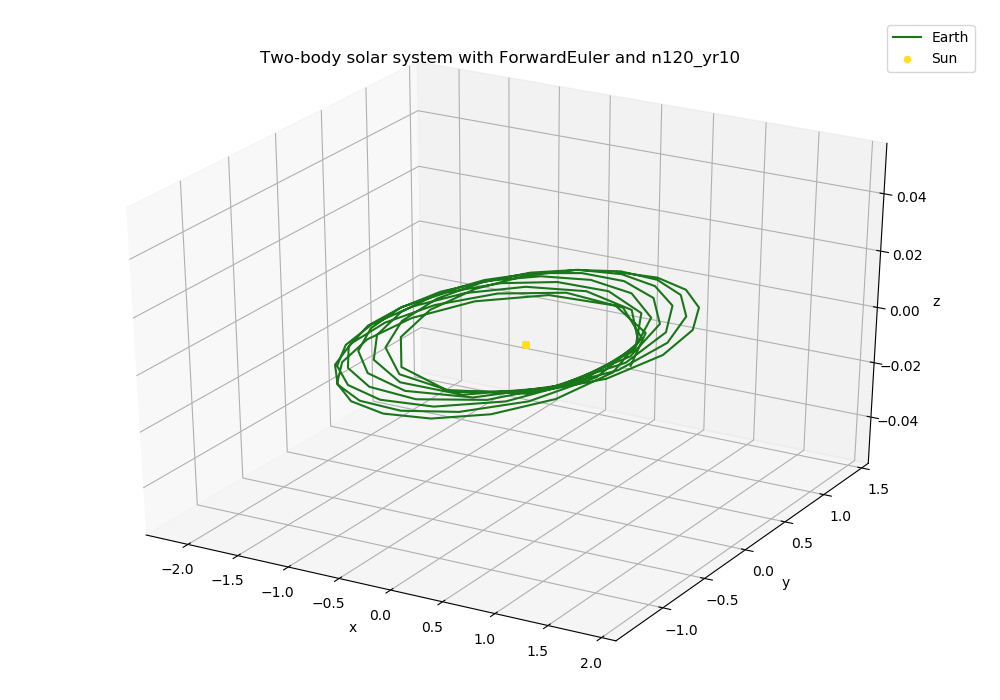
\includegraphics[width = 11cm]{img/plot3D_S_E_F_n120_yr10.png}
        \caption{Plot of the Sun-Earth solar system with 120 iterations over 10 years, made with Euler-Cromer. }
        \label{fig:plot3D_S_E_F_n120_yr10}
    \end{figure}

    \begin{figure}[H]
        \centering
        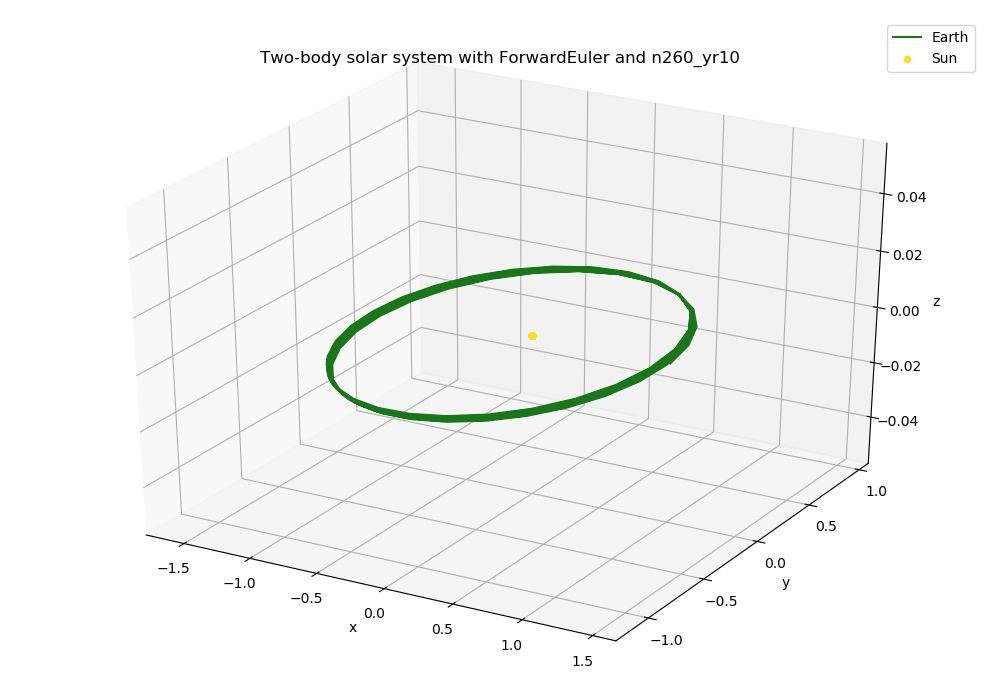
\includegraphics[width = 11cm]{img/plot3D_S_E_F_n260_yr10.png}
        \caption{Plot of the Sun-Earth solar system with 260 iterations over 10 years, made with Euler-Cromer. }
        \label{fig:plot3D_S_E_F_n260_yr10}
    \end{figure}

    \begin{figure}[H]
        \centering
        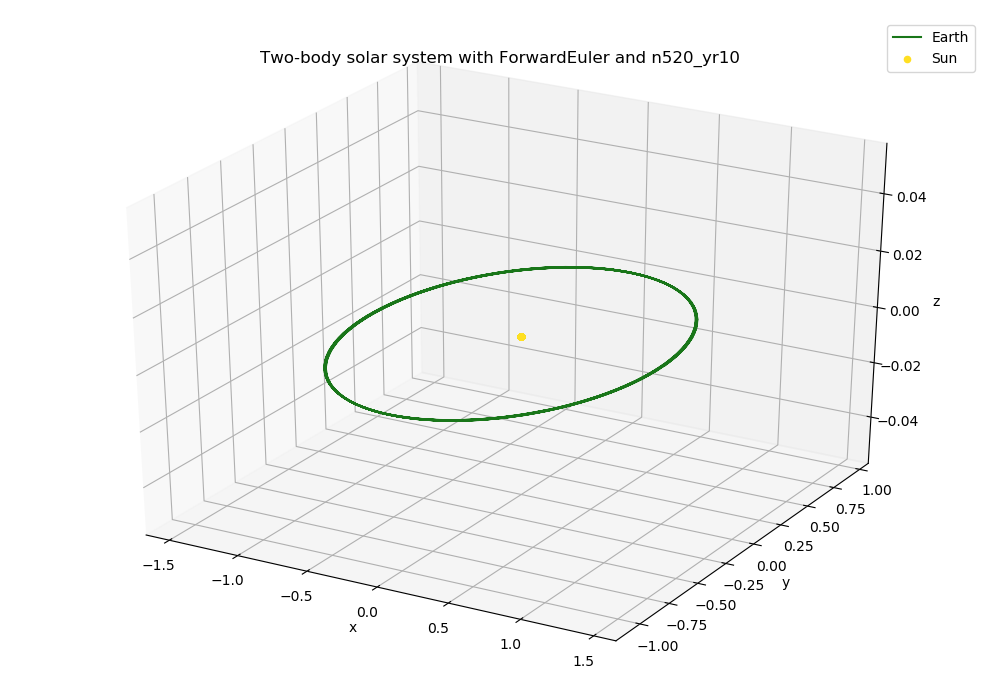
\includegraphics[width = 11cm]{img/plot3D_S_E_F_n520_yr10.png}
        \caption{Plot of the Sun-Earth solar system with 520 iterations over 10 years, made with Euler-Cromer. }
        \label{fig:plot3D_S_E_F_n520_yr10}
    \end{figure}

    \begin{figure}[H]
        \centering
        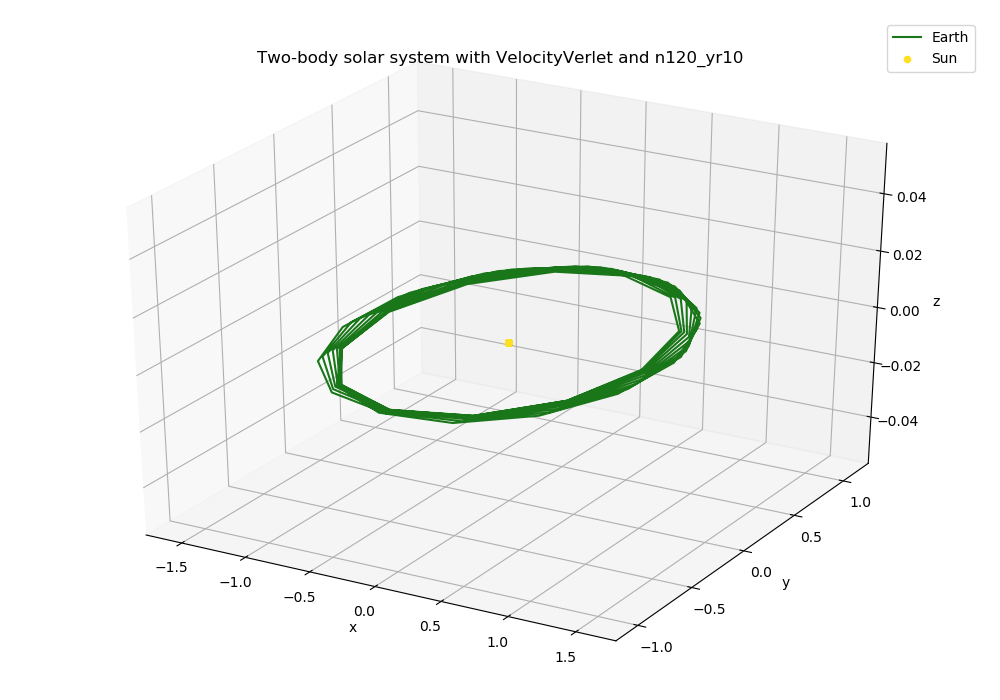
\includegraphics[width = 11cm]{img/plot3D_S_E_V_n120_yr10.png}
        \caption{Plot of the Sun-Earth solar system with 120 iterations over 10 years, made with Velocity Verlet. }
        \label{fig:plot3D_S_E_V_n120_yr10}
    \end{figure}

    \begin{figure}[H]
        \centering
        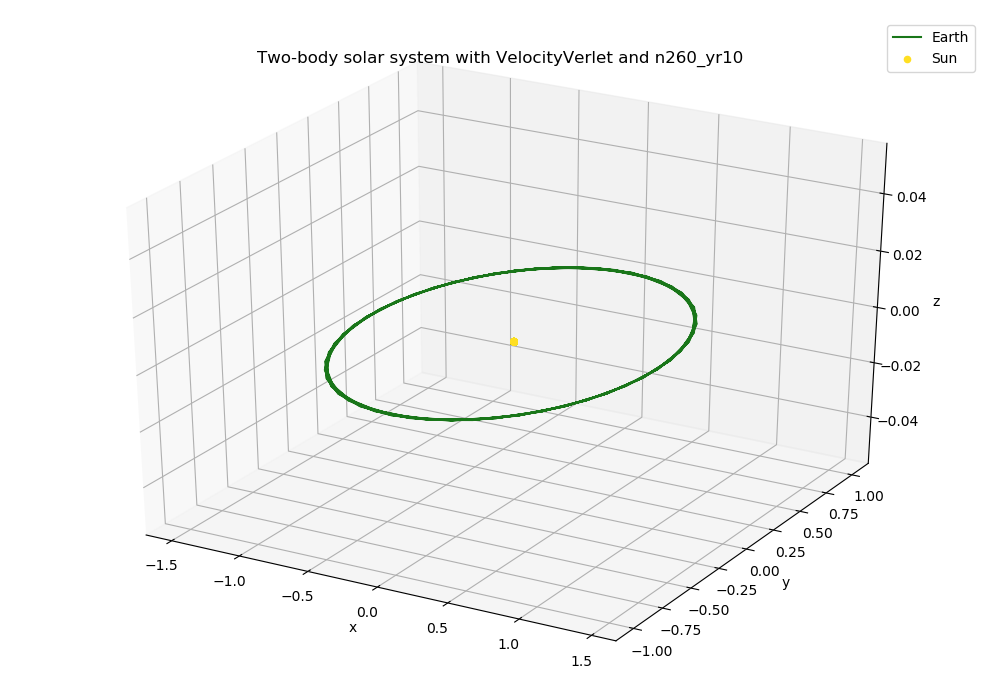
\includegraphics[width = 11cm]{img/plot3D_S_E_V_n260_yr10.png}
        \caption{Plot of the Sun-Earth solar system with 260 iterations over 10 years, made with Velocity Verlet. }
        \label{fig:plot3D_S_E_V_n260_yr10}
    \end{figure}

    \begin{figure}[H]
        \centering
        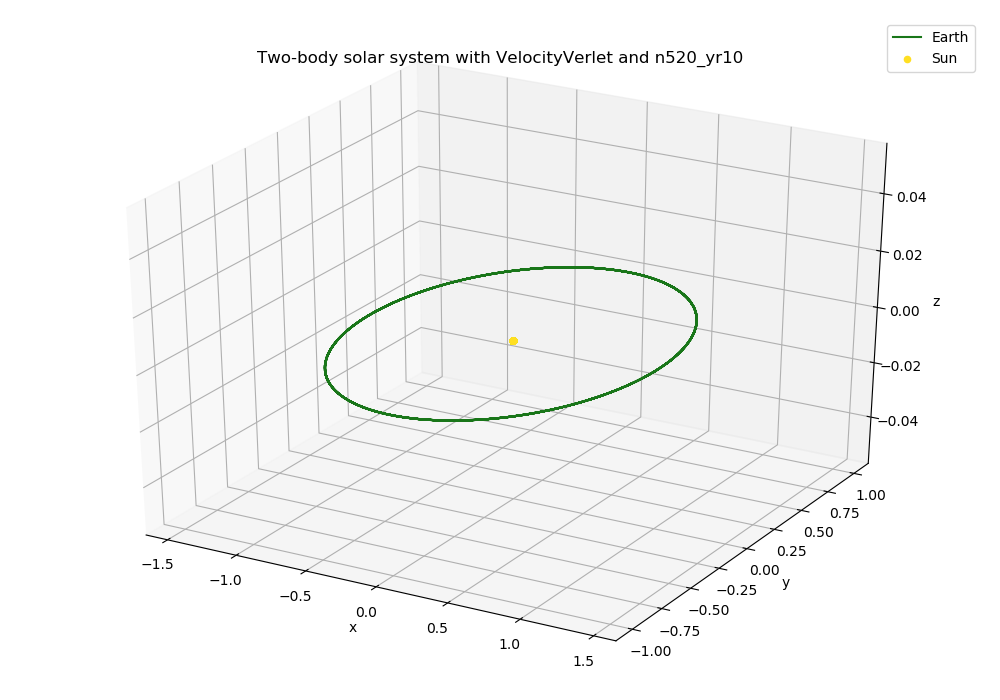
\includegraphics[width = 11cm]{img/plot3D_S_E_V_n520_yr10.png}
        \caption{Plot of the Sun-Earth solar system with 520 iterations over 10 years, made with Velocity Verlet. }
        \label{fig:plot3D_S_E_V_n520_yr10}
    \end{figure}

    \begin{table}[H]
        \centering
        \caption{Timings for the two methods for the ten-body solar system with 3660 iterations over 10 years.}
        \vspace{2mm}
        \label{tab:timings}
        \begin{tabular}{|c|c|}
            \hline
            Euler-Cromer time [s] & Velocity Verlet time [s] \\
            \hline \hline
            25.8553 & 34.0578 \\
            30.0186 & 30.5725 \\
            \hline
        \end{tabular} \\
        \hspace{0pt}\\
    \end{table}


\subsubsection{Testing the escape velocity}

    \begin{figure}[H]
        \centering
        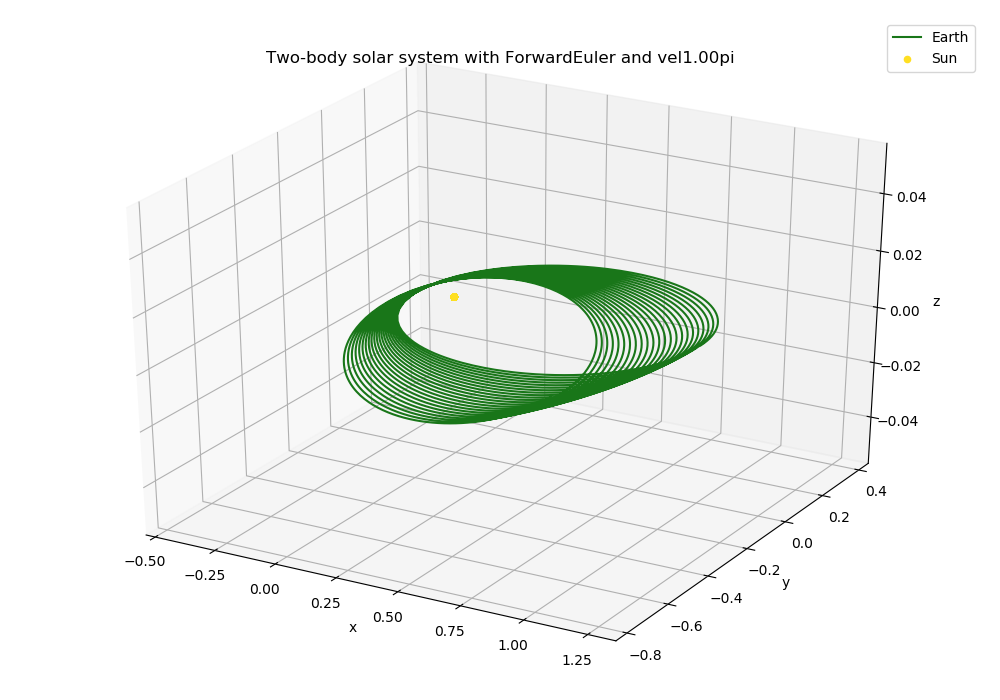
\includegraphics[width = 11cm]{img/plot3D_S_E_F_vel100pi.png}
        \caption{Plot of the Sun-Earth solar system with an escape velocity of $v_p = 1.00 \; \pi$ m/s, made with Euler-Cromer. }
        \label{fig:plot3D_S_E_F_vel100pi}
    \end{figure}

    \begin{figure}[H]
        \centering
        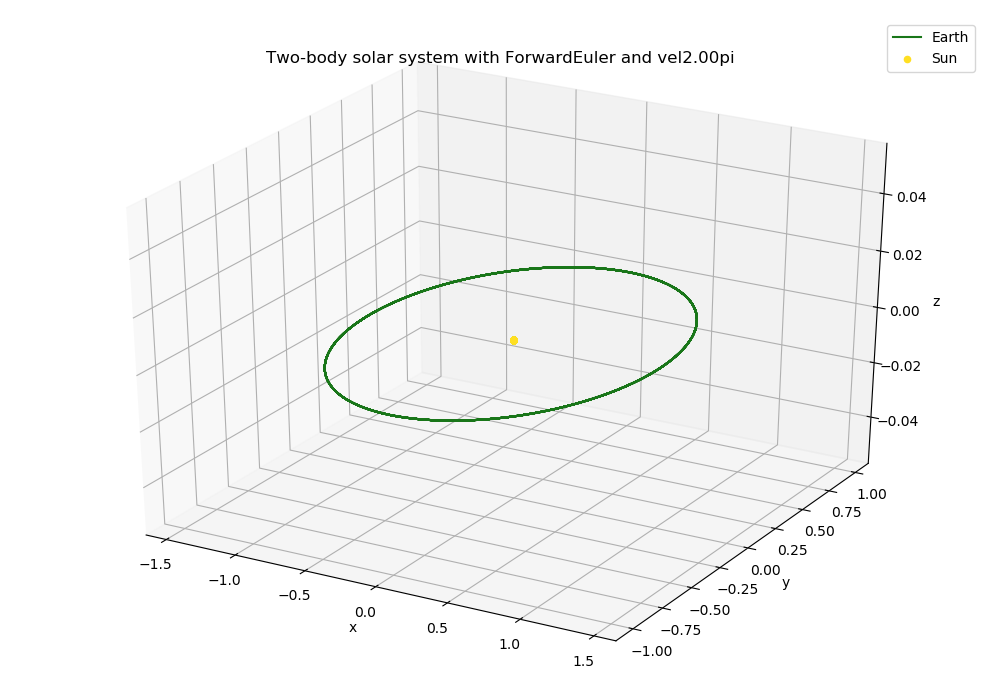
\includegraphics[width = 11cm]{img/plot3D_S_E_F_vel200pi.png}
        \caption{Plot of the Sun-Earth solar system with an escape velocity of $v_p = 2.00 \; \pi$ m/s, made with Euler-Cromer. }
        \label{fig:plot3D_S_E_F_vel200pi}
    \end{figure}

    \begin{figure}[H]
        \centering
        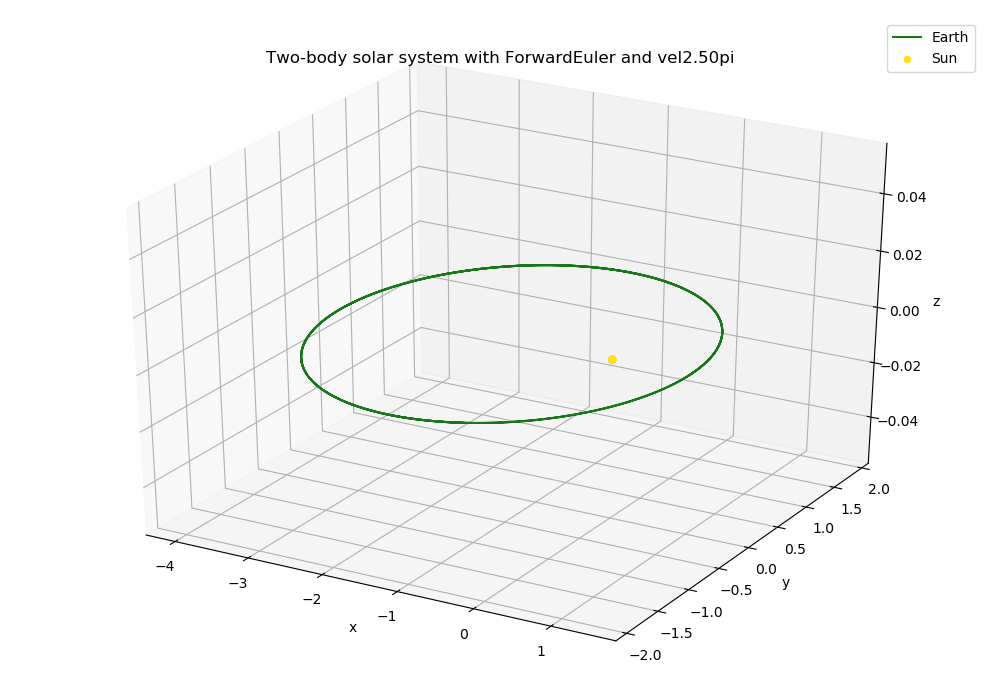
\includegraphics[width = 11cm]{img/plot3D_S_E_F_vel250pi.png}
        \caption{Plot of the Sun-Earth solar system with an escape velocity of $v_p = 2.50 \; \pi$ m/s, made with Euler-Cromer. }
        \label{fig:plot3D_S_E_F_vel250pi}
    \end{figure}

    \begin{figure}[H]
        \centering
        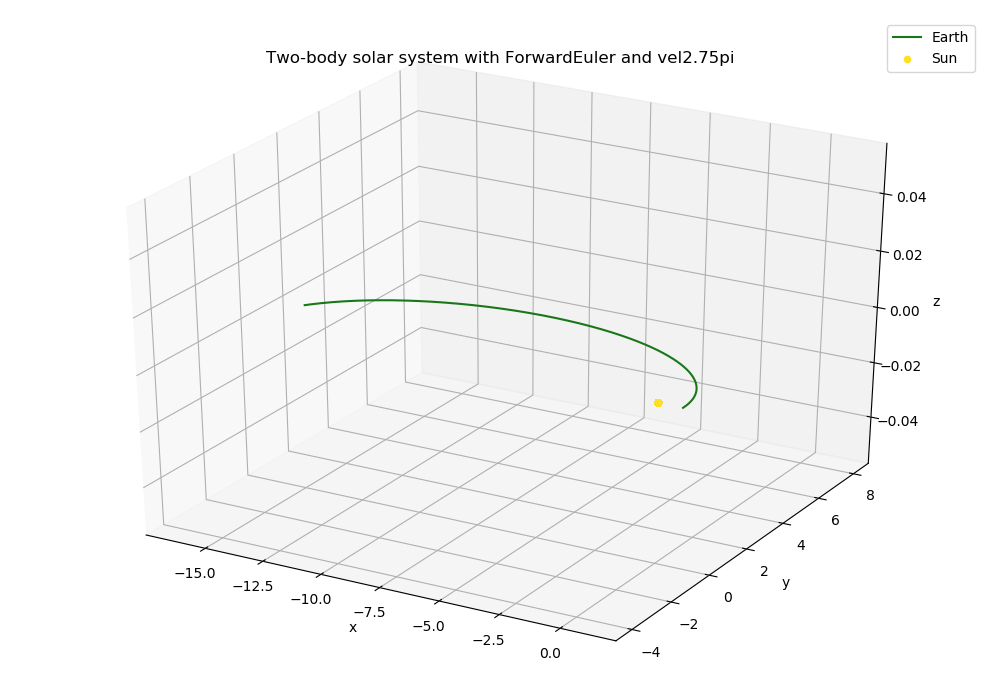
\includegraphics[width = 11cm]{img/plot3D_S_E_F_vel275pi.png}
        \caption{Plot of the Sun-Earth solar system with an escape velocity of $v_p = 2.75 \; \pi$ m/s, made with Euler-Cromer. }
        \label{fig:plot3D_S_E_F_vel275pi}
    \end{figure}

    \begin{figure}[H]
        \centering
        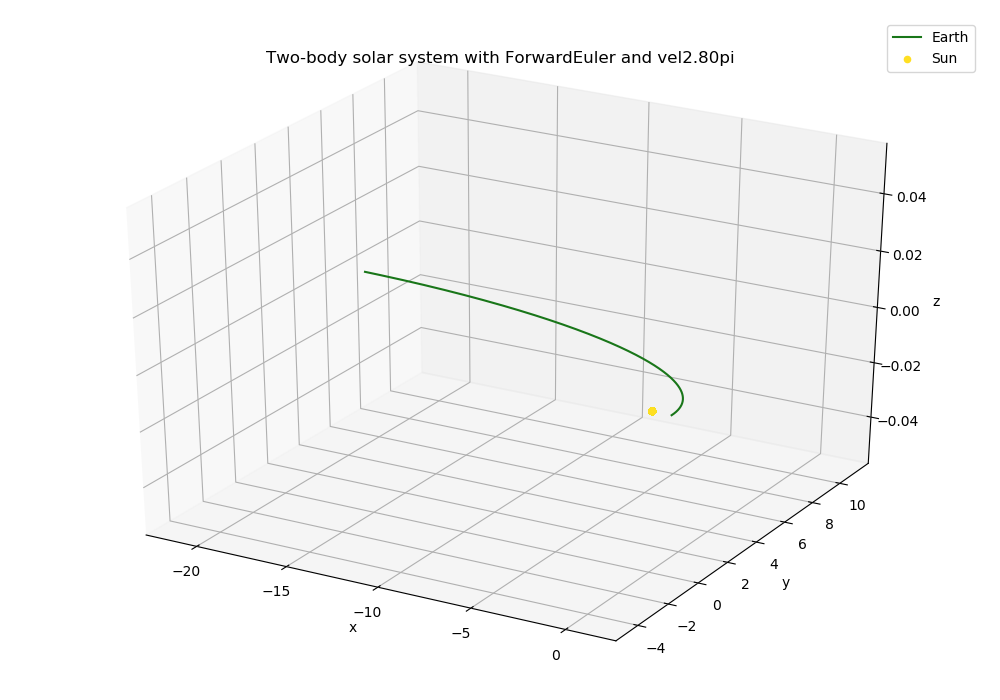
\includegraphics[width = 11cm]{img/plot3D_S_E_F_vel280pi.png}
        \caption{Plot of the Sun-Earth solar system with an escape velocity of $v_p = 2.80 \; \pi$ m/s, made with Euler-Cromer. }
        \label{fig:plot3D_S_E_F_vel280pi}
    \end{figure}

    \begin{figure}[H]
        \centering
        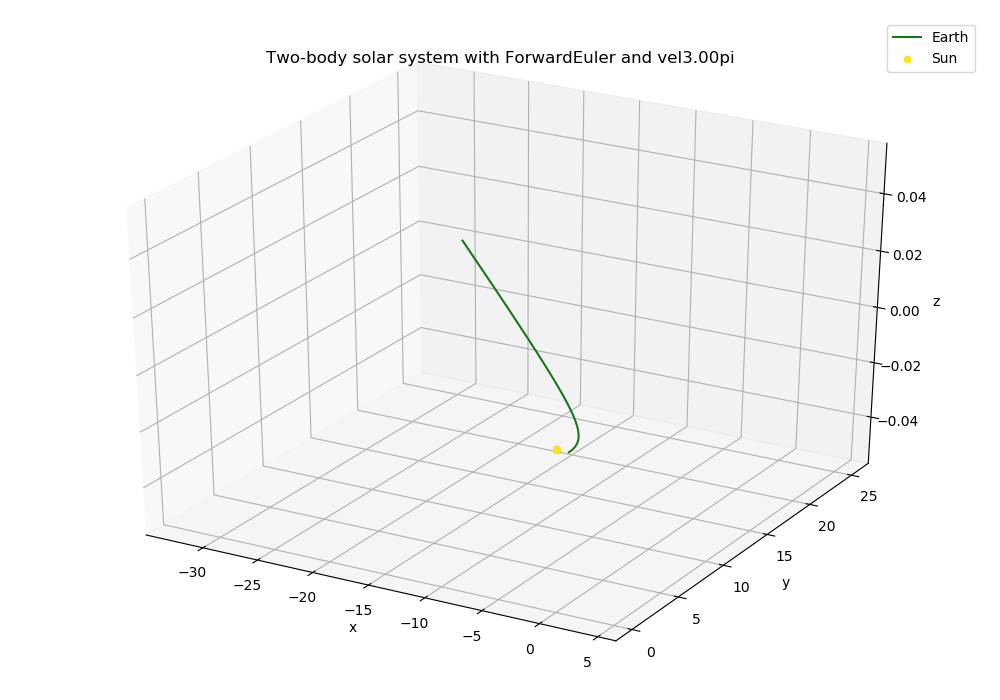
\includegraphics[width = 11cm]{img/plot3D_S_E_F_vel300pi.png}
        \caption{Plot of the Sun-Earth solar system with an escape velocity of $v_p = 3.00 \; \pi$ m/s, made with Euler-Cromer. }
        \label{fig:plot3D_S_E_F_vel300pi}
    \end{figure}

    \begin{figure}[H]
        \centering
        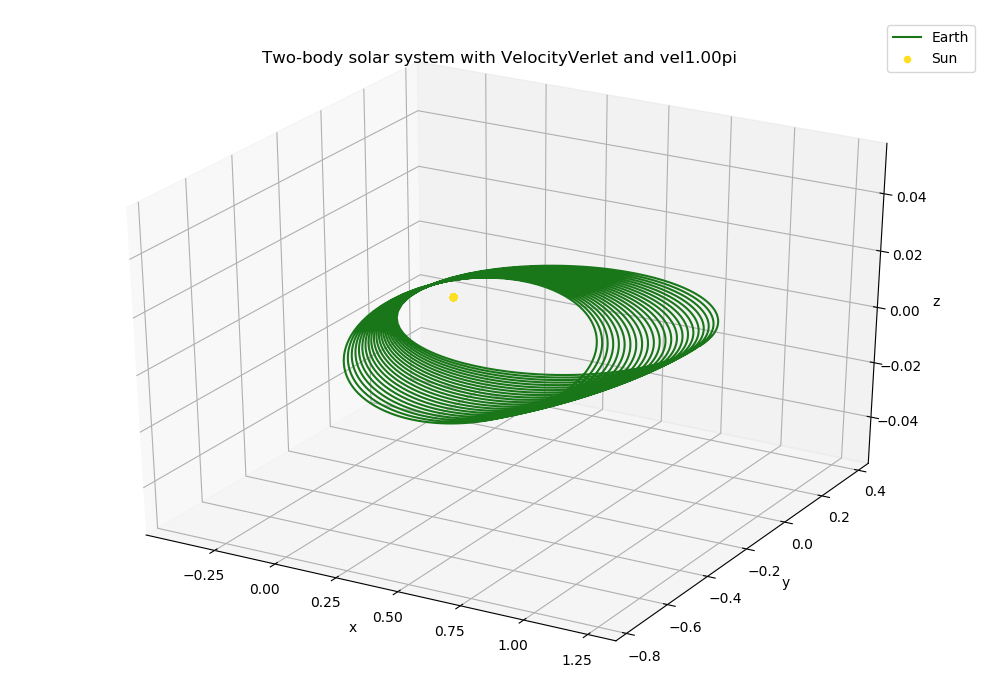
\includegraphics[width = 11cm]{img/plot3D_S_E_V_vel100pi.png}
        \caption{Plot of the Sun-Earth solar system with an escape velocity of $v_p = 1.00 \; \pi$ m/s, made with Velocity Verlet. }
        \label{fig:plot3D_S_E_V_vel100pi}
    \end{figure}

    \begin{figure}[H]
        \centering
        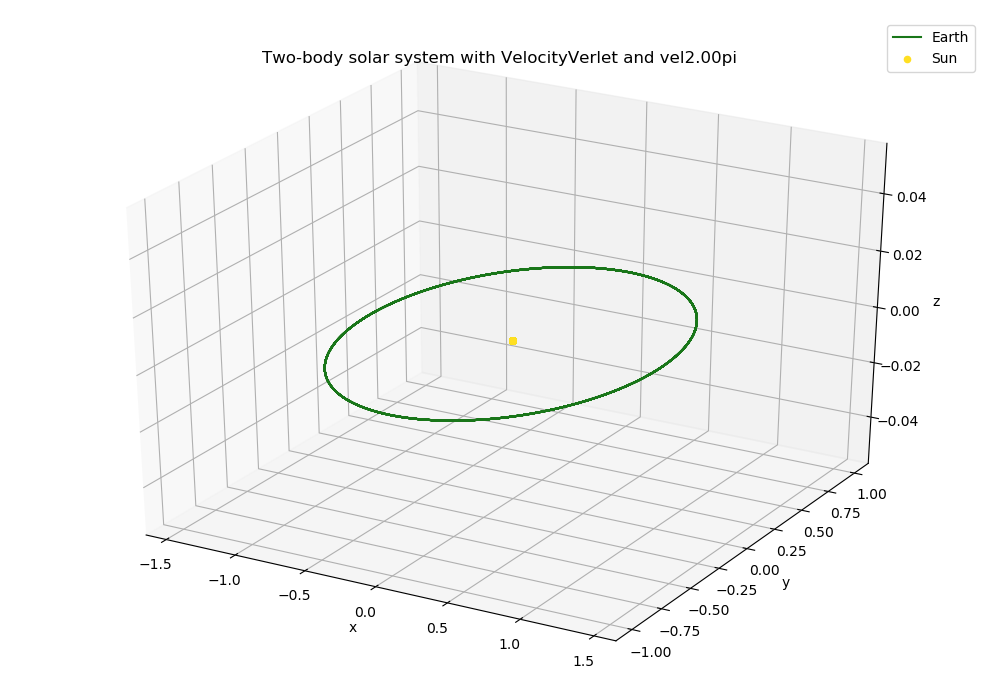
\includegraphics[width = 11cm]{img/plot3D_S_E_V_vel200pi.png}
        \caption{Plot of the Sun-Earth solar system with an escape velocity of $v_p = 2.00 \; \pi$ m/s, made with Velocity Verlet. }
        \label{fig:plot3D_S_E_V_vel200pi}
    \end{figure}

    \begin{figure}[H]
        \centering
        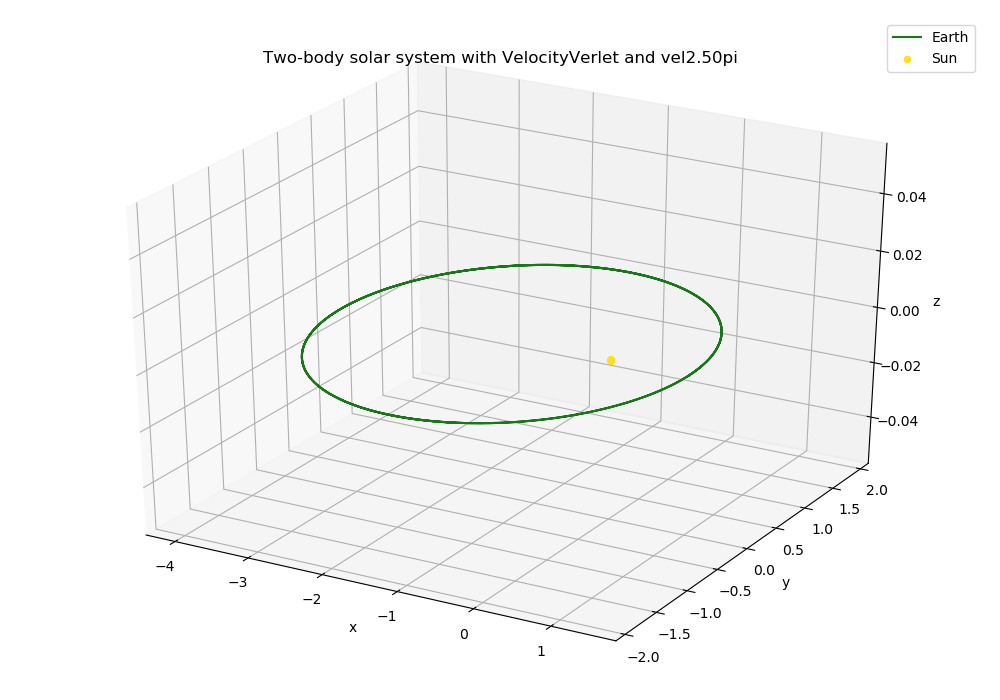
\includegraphics[width = 11cm]{img/plot3D_S_E_V_vel250pi.png}
        \caption{Plot of the Sun-Earth solar system with an escape velocity of $v_p = 2.50 \; \pi$ m/s, made with Velocity Verlet. }
        \label{fig:plot3D_S_E_V_vel250pi}
    \end{figure}

    \begin{figure}[H]
        \centering
        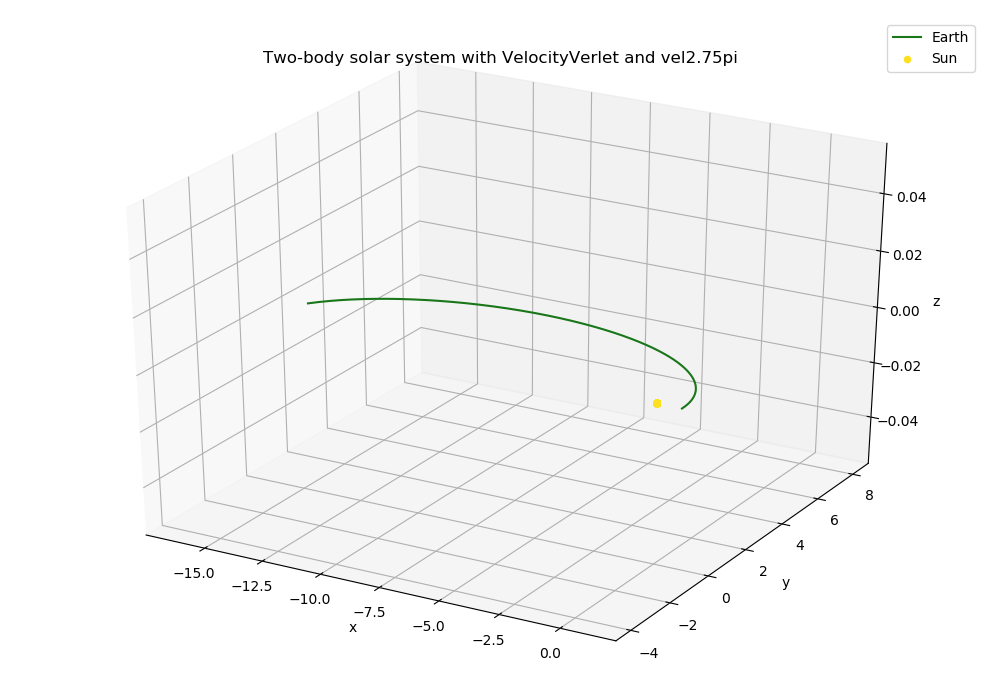
\includegraphics[width = 11cm]{img/plot3D_S_E_V_vel275pi.png}
        \caption{Plot of the Sun-Earth solar system with an escape velocity of $v_p = 2.75 \; \pi$ m/s, made with Velocity Verlet. }
        \label{fig:plot3D_S_E_V_vel275pi}
    \end{figure}

    \begin{figure}[H]
        \centering
        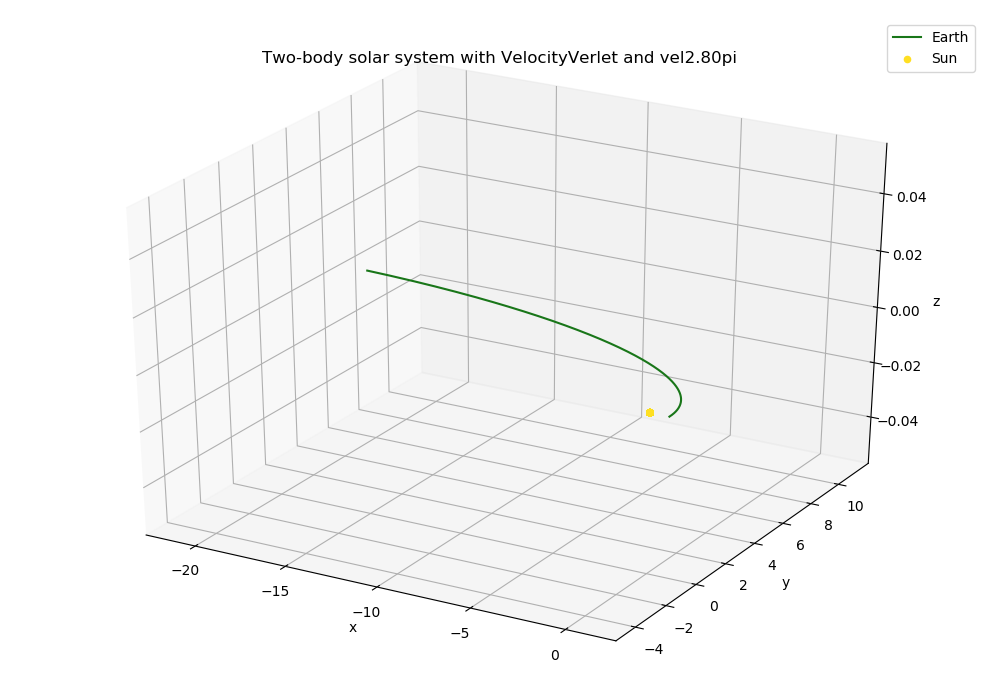
\includegraphics[width = 11cm]{img/plot3D_S_E_V_vel280pi.png}
        \caption{Plot of the Sun-Earth solar system with an escape velocity of $v_p = 2.80 \; \pi$ m/s, made with Velocity Verlet. }
        \label{fig:plot3D_S_E_V_vel280pi}
    \end{figure}

    \begin{figure}[H]
        \centering
        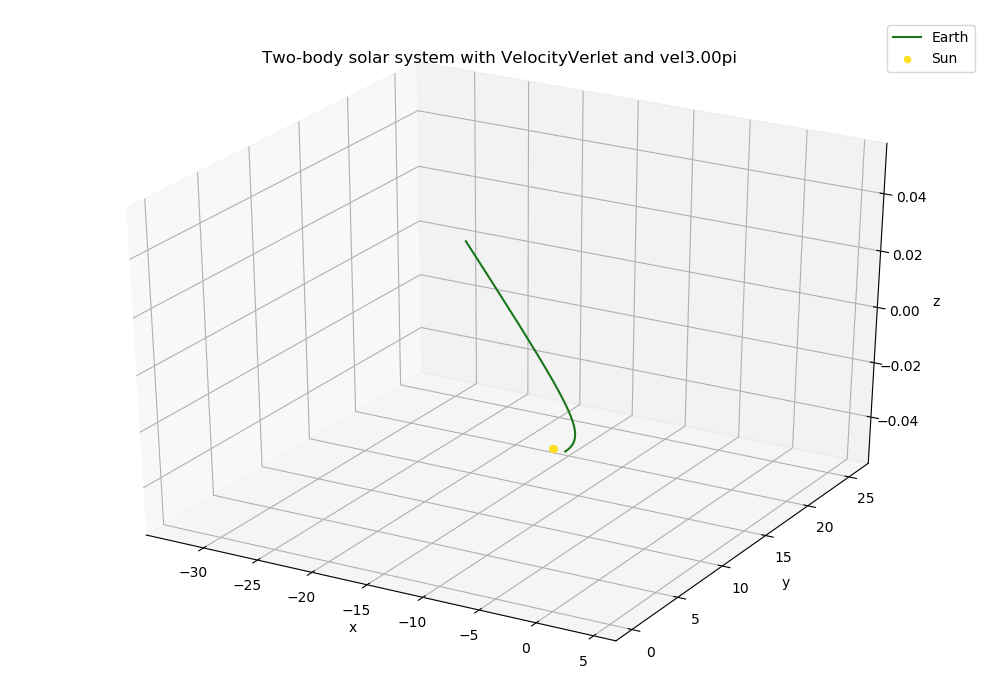
\includegraphics[width = 11cm]{img/plot3D_S_E_V_vel300pi.png}
        \caption{Plot of the Sun-Earth solar system with an escape velocity of $v_p = 3.00 \; \pi$ m/s, made with Velocity Verlet. }
        \label{fig:plot3D_S_E_V_vel300pi}
    \end{figure}

\subsubsection{Testing different values of \texorpdfstring{$\beta$}{TEXT}}

    \begin{figure}[H]
        \centering
        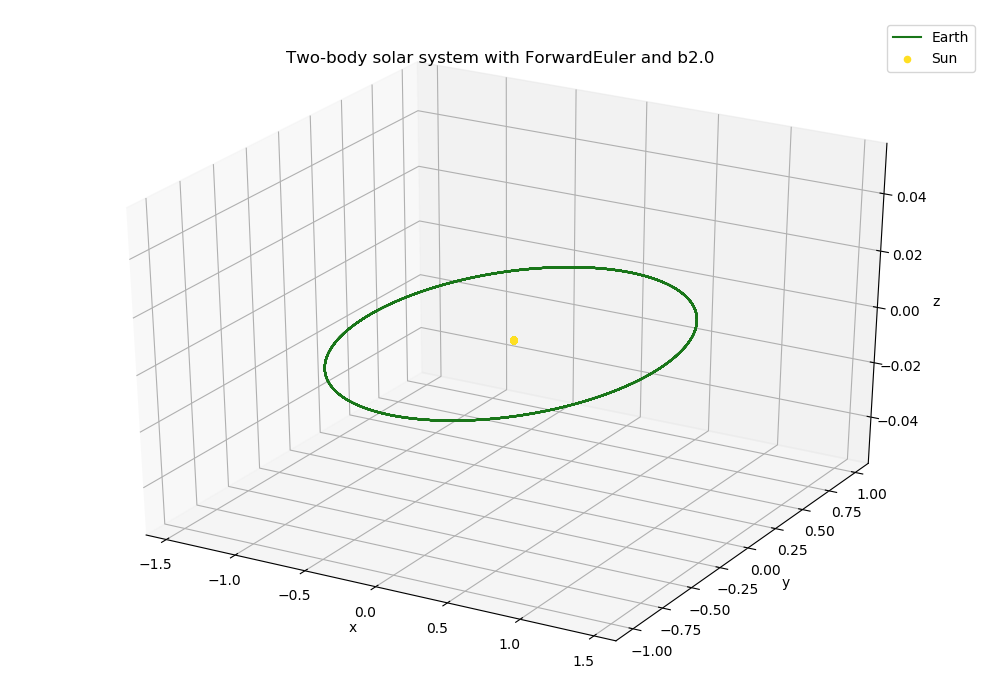
\includegraphics[width = 11cm]{img/plot3D_S_E_F_b20.png}
        \caption{Plot of the Sun-Earth solar system with $\beta = 2.0$, made with Euler-Cromer. }
        \label{fig:plot3D_S_E_F_b20}
    \end{figure}

    \begin{figure}[H]
        \centering
        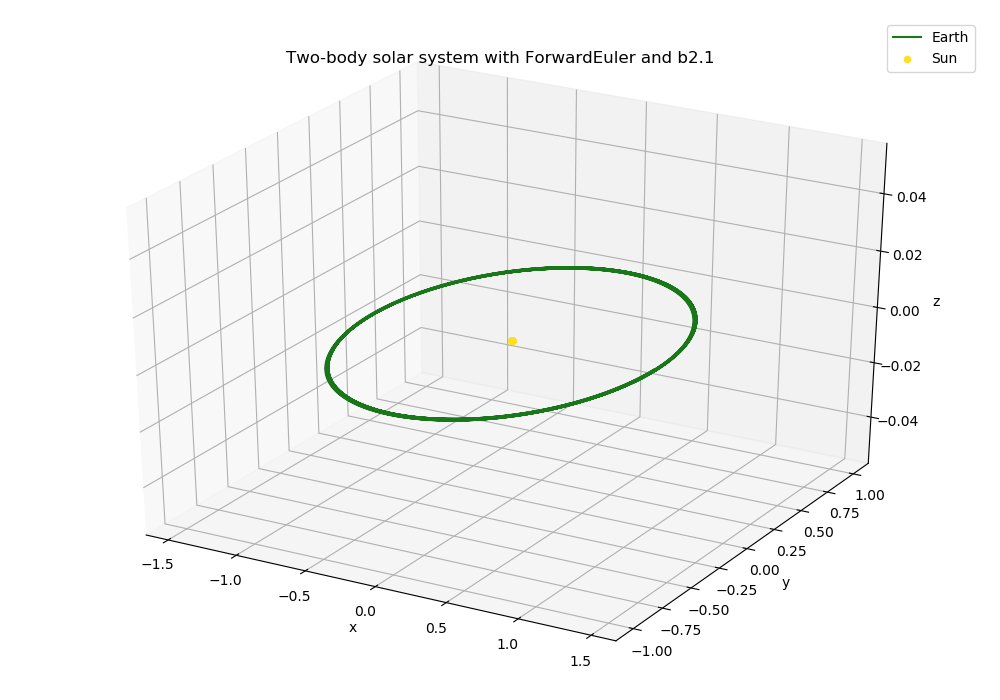
\includegraphics[width = 11cm]{img/plot3D_S_E_F_b21.png}
        \caption{Plot of the Sun-Earth solar system with $\beta = 2.1$, made with Euler-Cromer.}
        \label{fig:plot3D_S_E_F_b21}
    \end{figure}

    \begin{figure}[H]
        \centering
        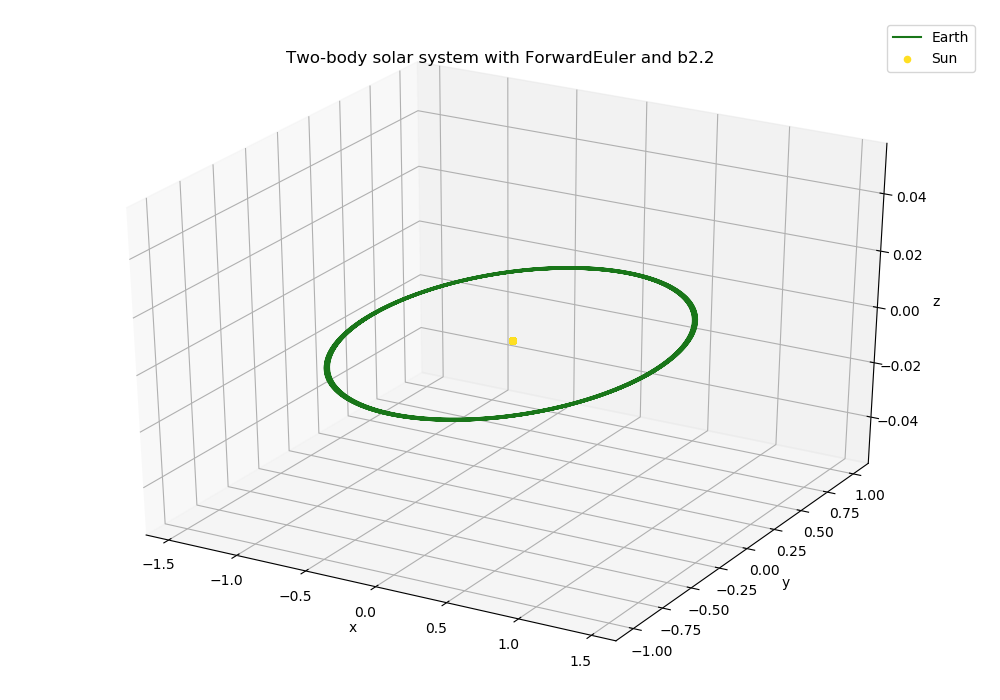
\includegraphics[width = 11cm]{img/plot3D_S_E_F_b22.png}
        \caption{Plot of the Sun-Earth solar system with $\beta = 2.2$, made with Euler-Cromer.}
        \label{fig:plot3D_S_E_F_b22}
    \end{figure}

    \begin{figure}[H]
        \centering
        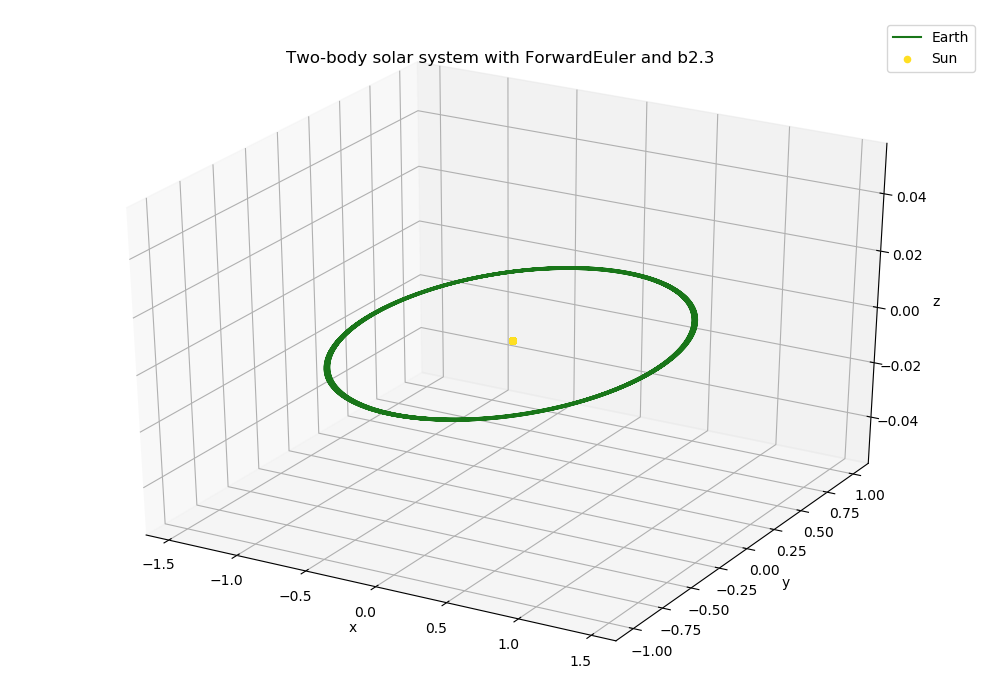
\includegraphics[width = 11cm]{img/plot3D_S_E_F_b23.png}
        \caption{Plot of the Sun-Earth solar system with $\beta = 2.3$, made with Euler-Cromer.}
        \label{fig:plot3D_S_E_F_b23}
    \end{figure}

    \begin{figure}[H]
        \centering
        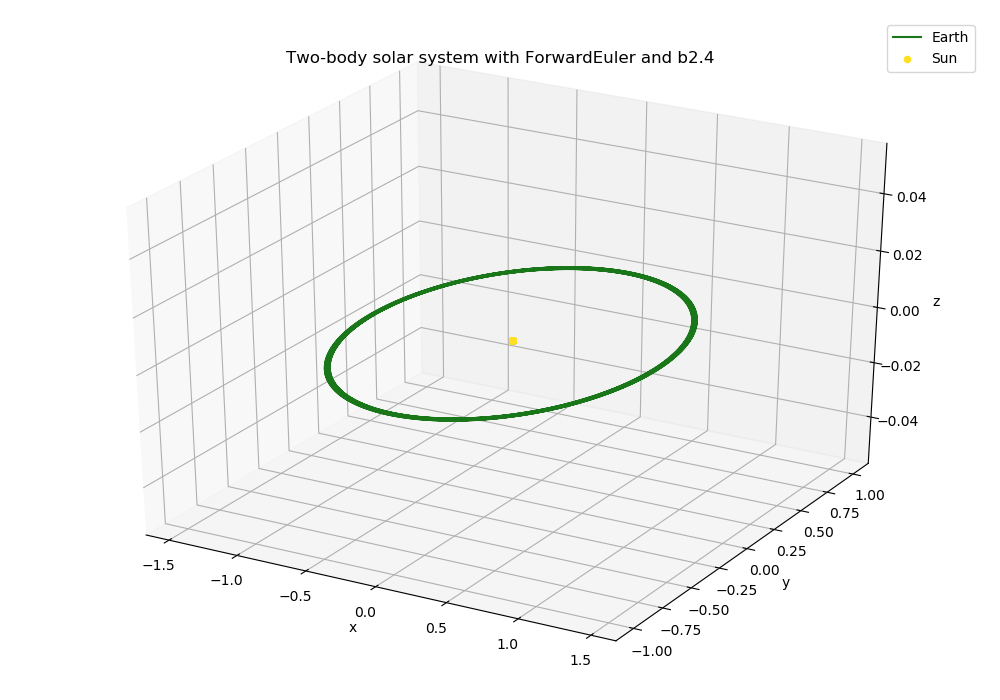
\includegraphics[width = 11cm]{img/plot3D_S_E_F_b24.png}
        \caption{Plot of the Sun-Earth solar system with $\beta = 2.4$, made with Euler-Cromer.}
        \label{fig:plot3D_S_E_F_b24}
    \end{figure}

    \begin{figure}[H]
        \centering
        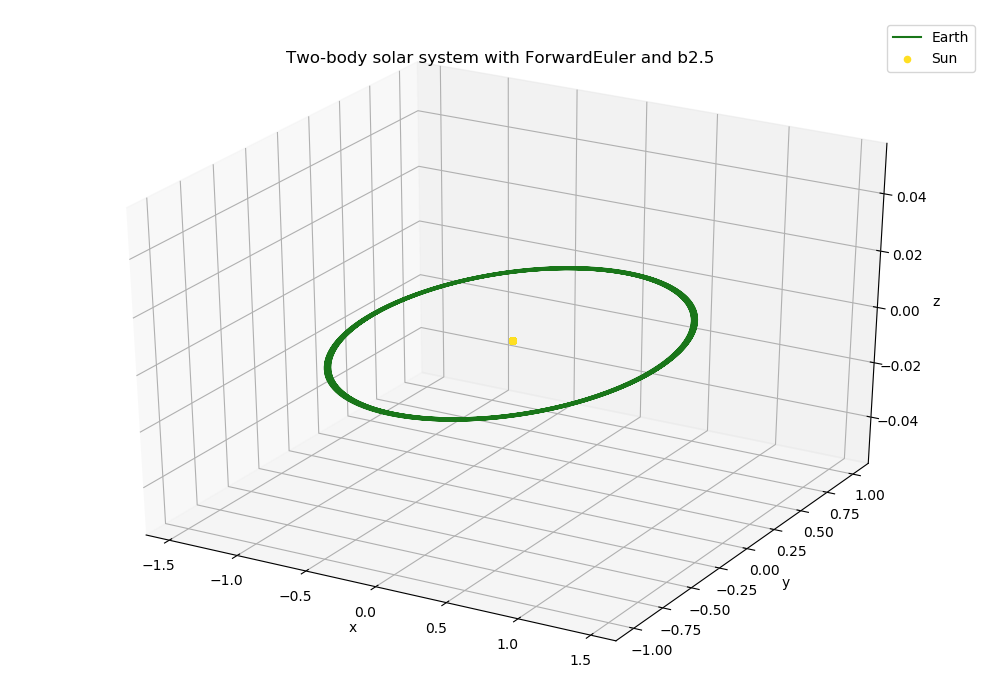
\includegraphics[width = 11cm]{img/plot3D_S_E_F_b25.png}
        \caption{Plot of the Sun-Earth solar system with $\beta = 2.5$, made with Euler-Cromer.}
        \label{fig:plot3D_S_E_F_b25}
    \end{figure}

    \begin{figure}[H]
        \centering
        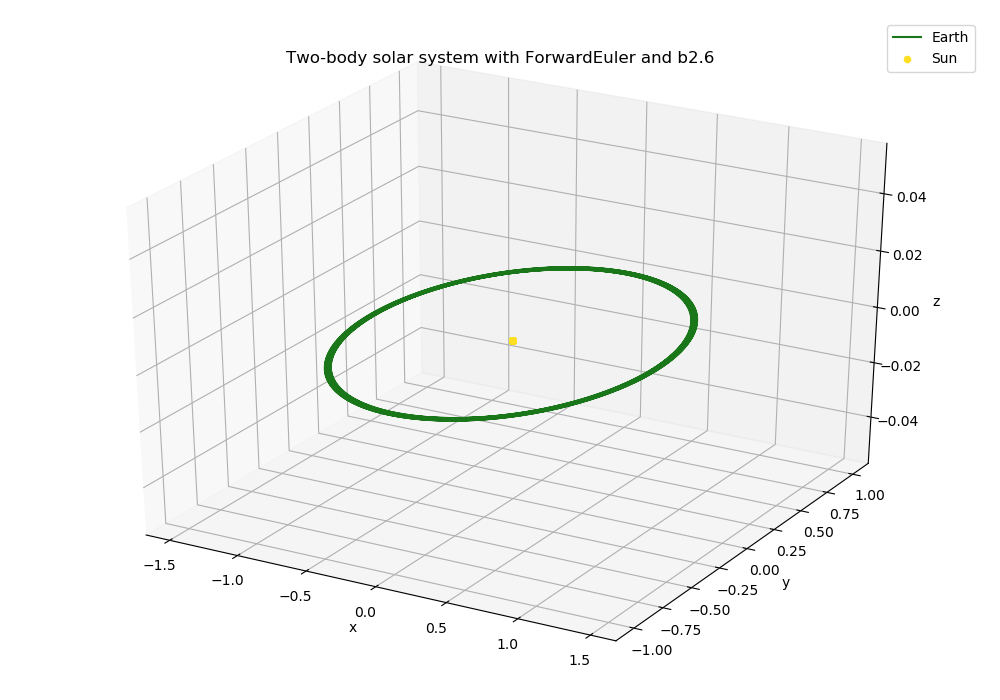
\includegraphics[width = 11cm]{img/plot3D_S_E_F_b26.png}
        \caption{Plot of the Sun-Earth solar system with $\beta = 2.6$, made with Euler-Cromer.}
        \label{fig:plot3D_S_E_F_b26}
    \end{figure}

    \begin{figure}[H]
        \centering
        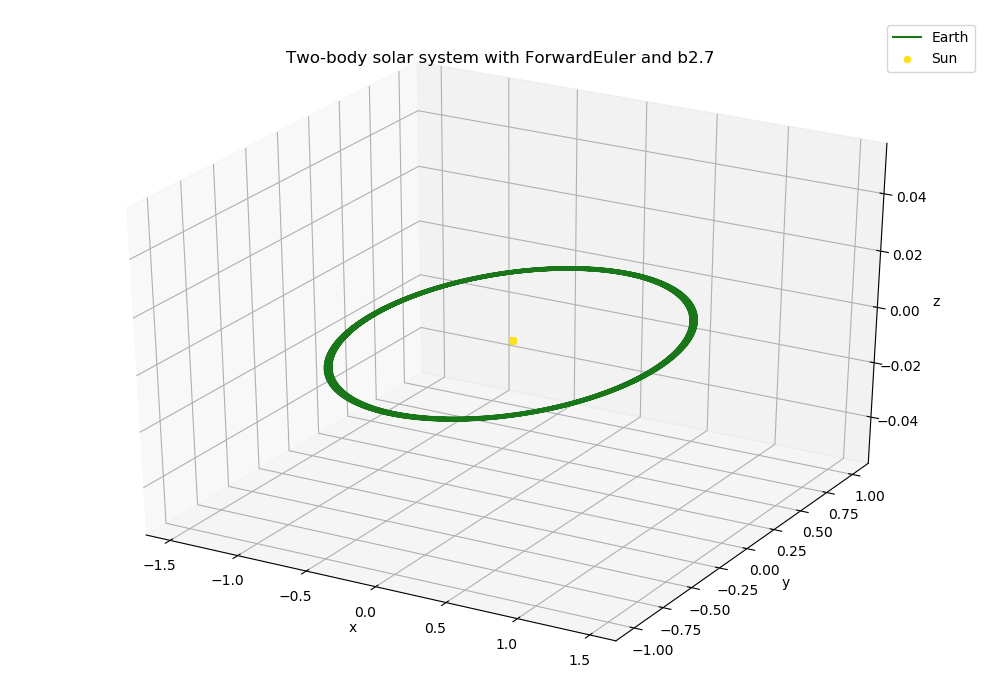
\includegraphics[width = 11cm]{img/plot3D_S_E_F_b27.png}
        \caption{Plot of the Sun-Earth solar system with $\beta = 2.7$, made with Euler-Cromer.}
        \label{fig:plot3D_S_E_F_b27}
    \end{figure}

    \begin{figure}[H]
        \centering
        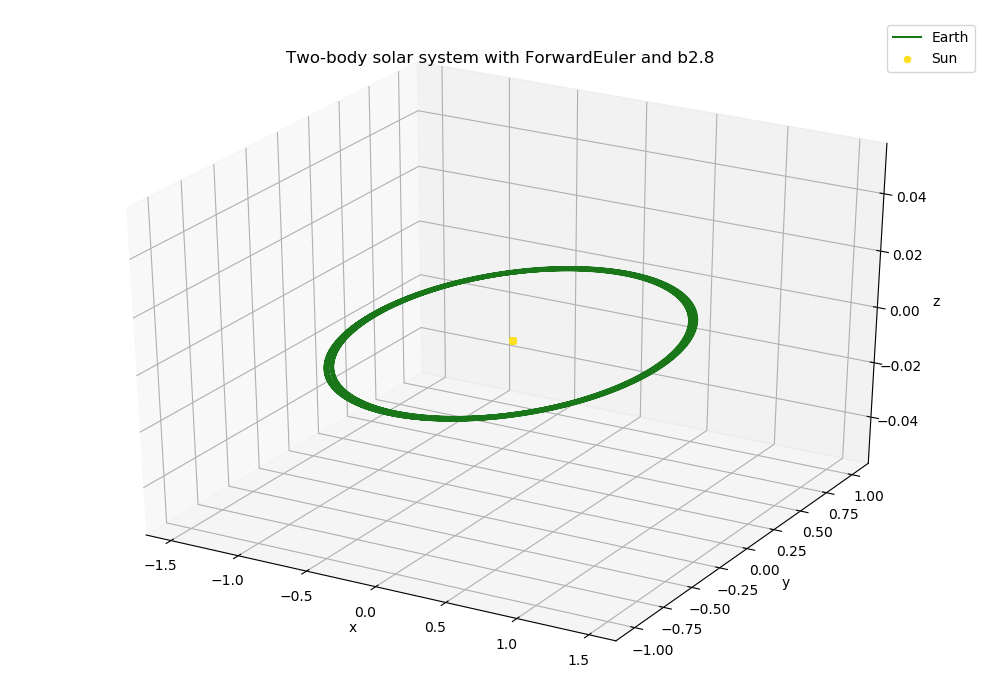
\includegraphics[width = 11cm]{img/plot3D_S_E_F_b28.png}
        \caption{Plot of the Sun-Earth solar system with $\beta = 2.8$, made with Euler-Cromer.}
        \label{fig:plot3D_S_E_F_b28}
    \end{figure}

    \begin{figure}[H]
        \centering
        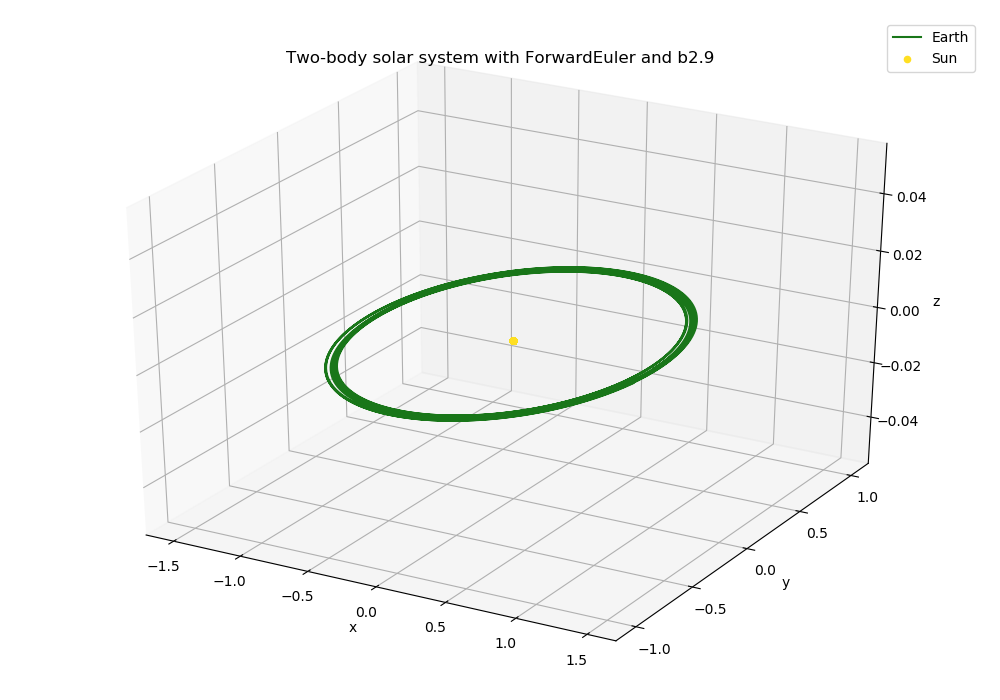
\includegraphics[width = 11cm]{img/plot3D_S_E_F_b29.png}
        \caption{Plot of the Sun-Earth solar system with $\beta = 2.9$, made with Euler-Cromer.}
        \label{fig:plot3D_S_E_F_b29}
    \end{figure}

    \begin{figure}[H]
        \centering
        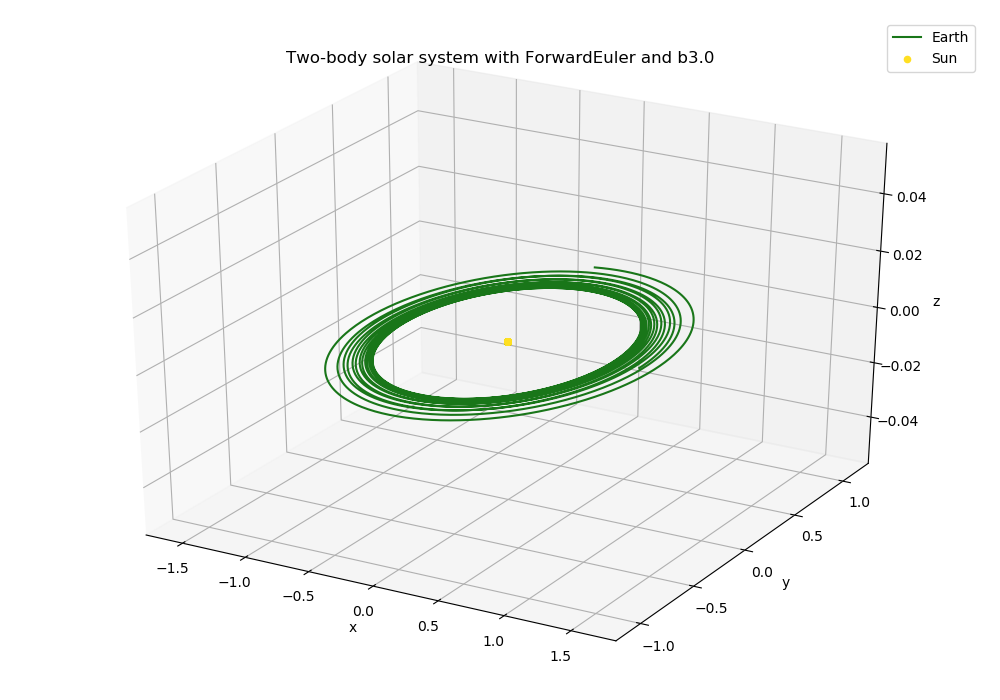
\includegraphics[width = 11cm]{img/plot3D_S_E_F_b30.png}
        \caption{Plot of the Sun-Earth solar system with $\beta = 3.0$, made with Euler-Cromer.}
        \label{fig:plot3D_S_E_F_b30}
    \end{figure}

    \begin{figure}[H]
        \centering
        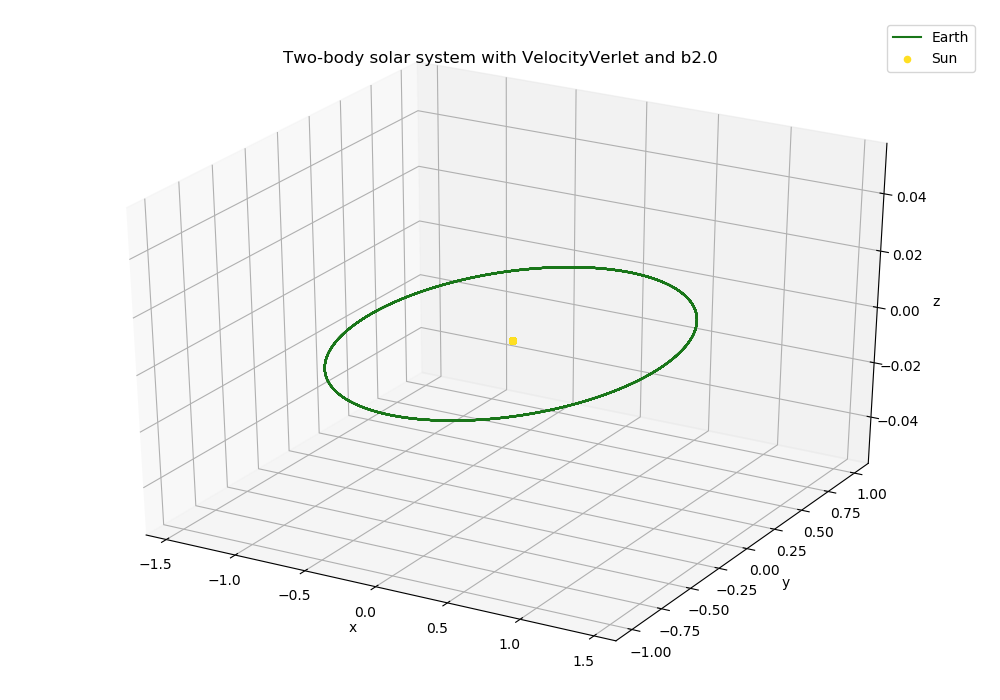
\includegraphics[width = 11cm]{img/plot3D_S_E_V_b20.png}
        \caption{Plot of the Sun-Earth solar system with $\beta = 2.0$, made with Velocity Verlet.}
        \label{fig:plot3D_S_E_V_b20}
    \end{figure}

    \begin{figure}[H]
        \centering
        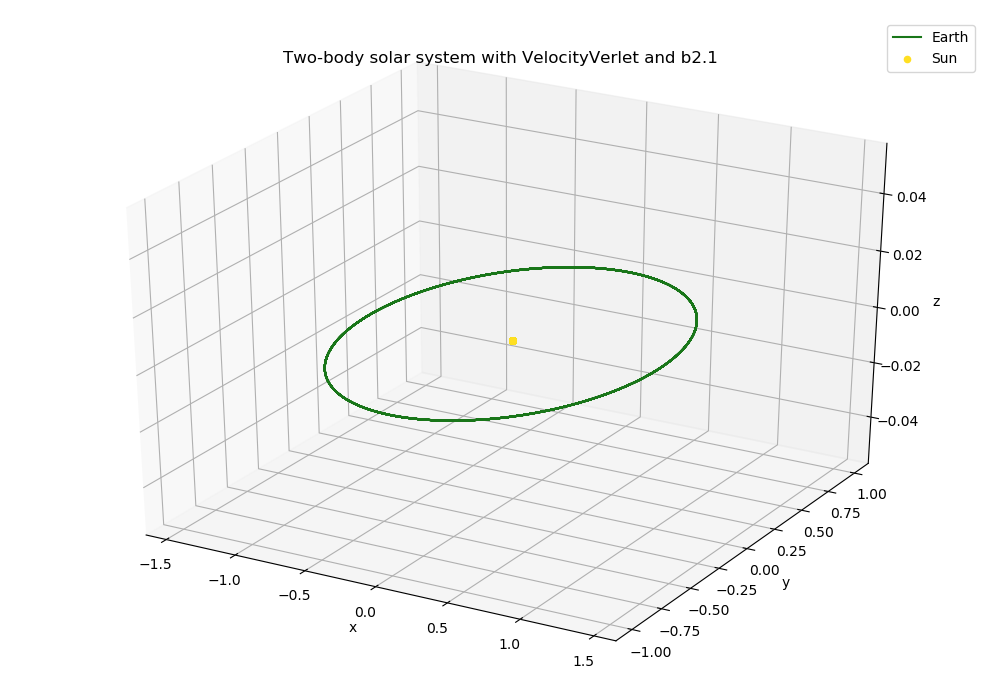
\includegraphics[width = 11cm]{img/plot3D_S_E_V_b21.png}
        \caption{Plot of the Sun-Earth solar system with $\beta = 2.1$, made with Velocity Verlet.}
        \label{fig:plot3D_S_E_V_b21}
    \end{figure}

    \begin{figure}[H]
        \centering
        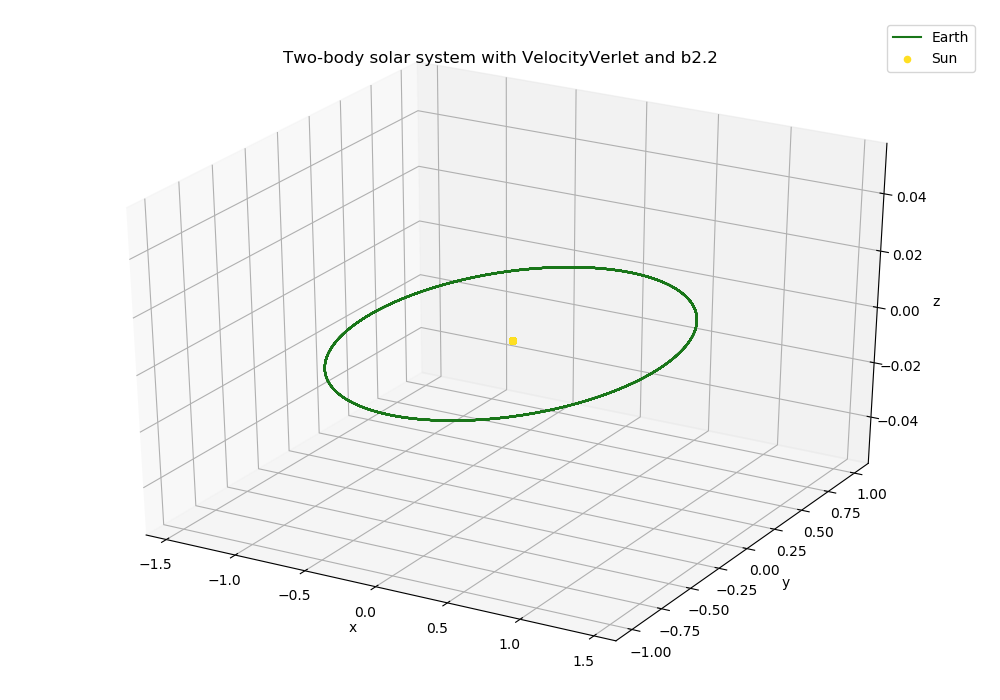
\includegraphics[width = 11cm]{img/plot3D_S_E_V_b22.png}
        \caption{Plot of the Sun-Earth solar system with $\beta = 2.2$, made with Velocity Verlet.}
        \label{fig:plot3D_S_E_V_b22}
    \end{figure}

    \begin{figure}[H]
        \centering
        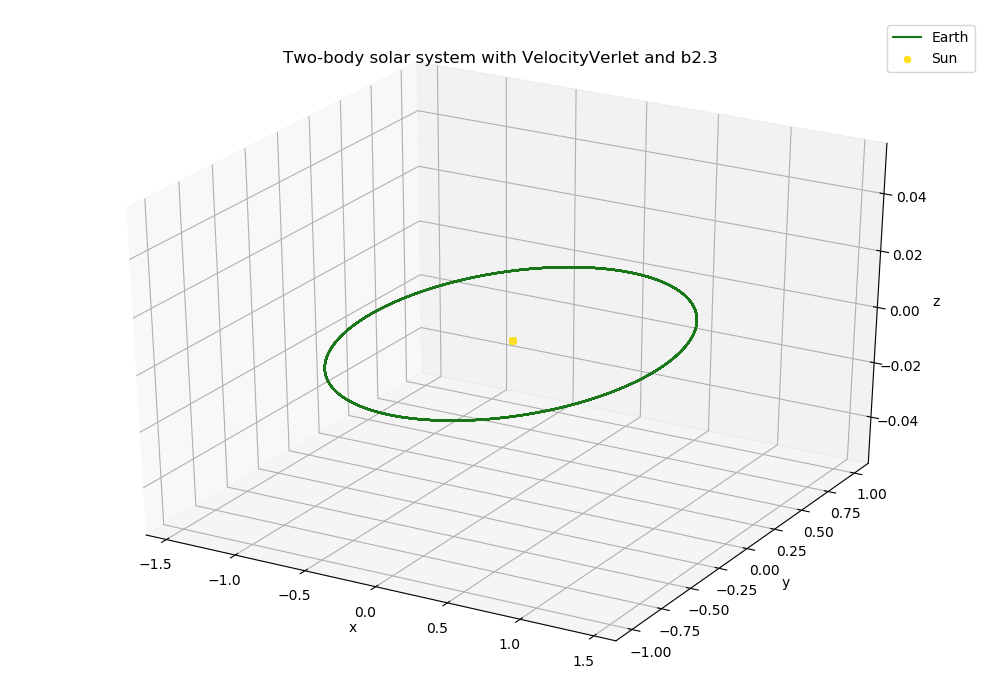
\includegraphics[width = 11cm]{img/plot3D_S_E_V_b23.png}
        \caption{Plot of the Sun-Earth solar system with $\beta = 2.3$, made with Velocity Verlet.}
        \label{fig:plot3D_S_E_V_b23}
    \end{figure}

    \begin{figure}[H]
        \centering
        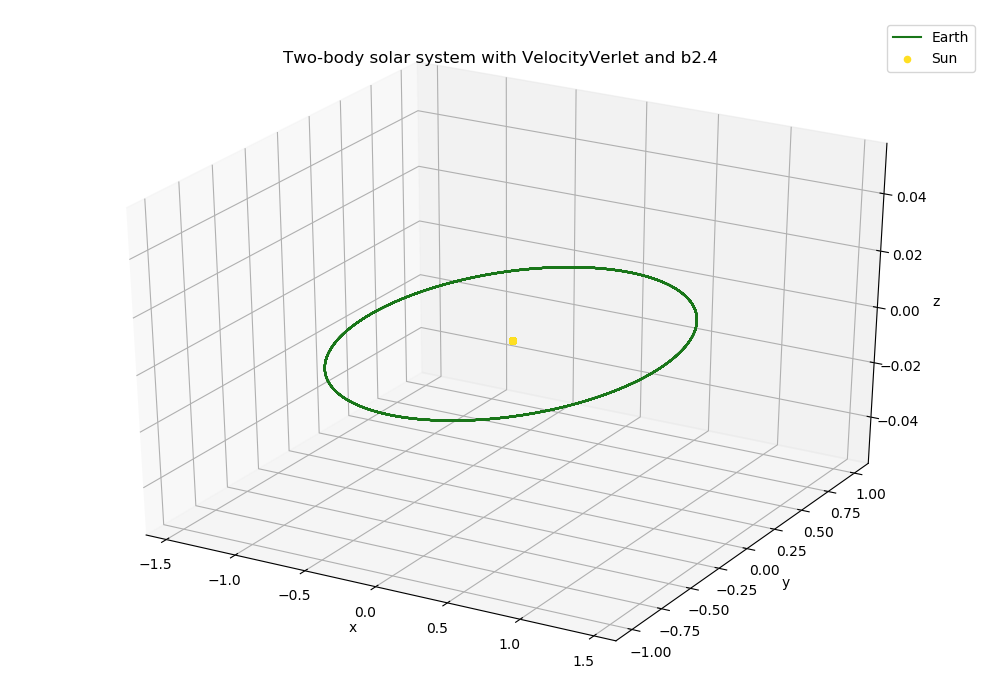
\includegraphics[width = 11cm]{img/plot3D_S_E_V_b24.png}
        \caption{Plot of the Sun-Earth solar system with $\beta = 2.4$, made with Velocity Verlet.}
        \label{fig:plot3D_S_E_V_b24}
    \end{figure}

    \begin{figure}[H]
        \centering
        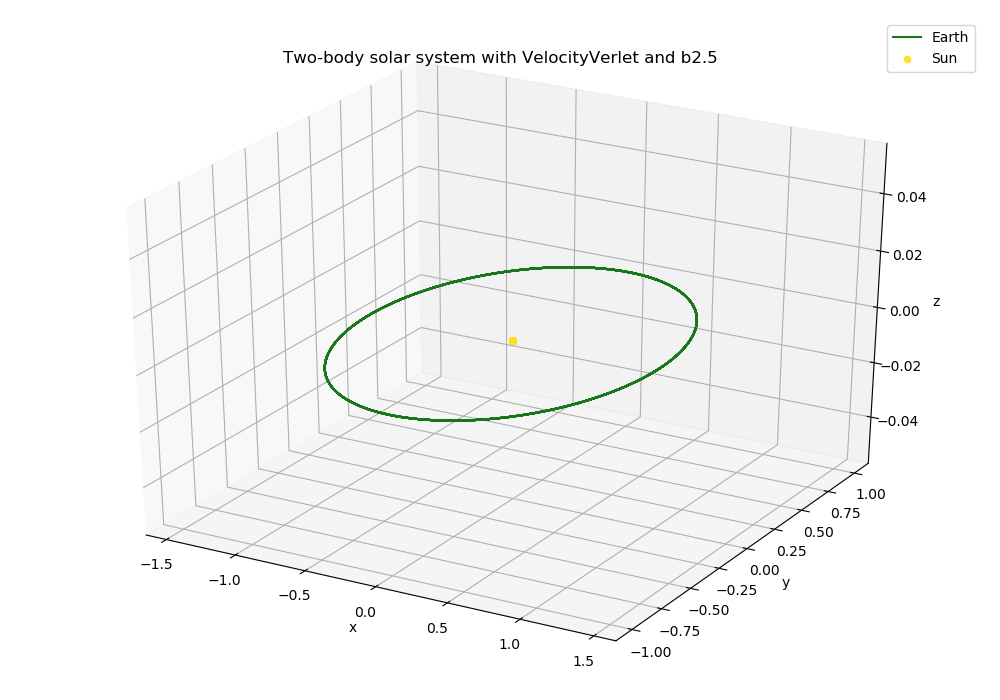
\includegraphics[width = 11cm]{img/plot3D_S_E_V_b25.png}
        \caption{Plot of the Sun-Earth solar system with $\beta = 2.5$, made with Velocity Verlet.}
        \label{fig:plot3D_S_E_V_b25}
    \end{figure}

    \begin{figure}[H]
        \centering
        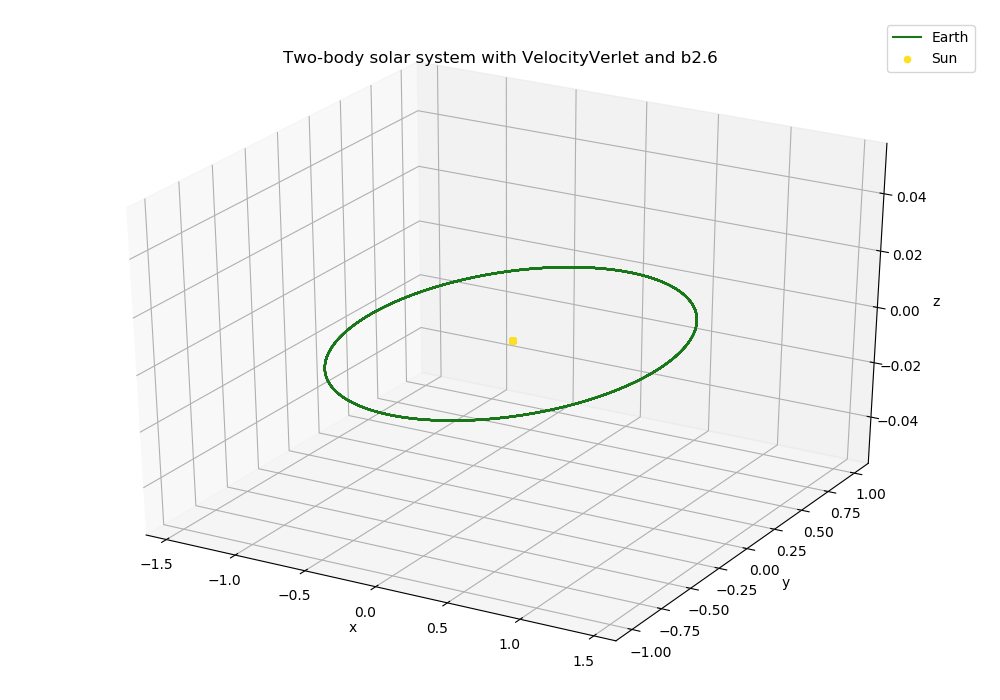
\includegraphics[width = 11cm]{img/plot3D_S_E_V_b26.png}
        \caption{Plot of the Sun-Earth solar system with $\beta = 2.6$, made with Velocity Verlet.}
        \label{fig:plot3D_S_E_V_b26}
    \end{figure}

    \begin{figure}[H]
        \centering
        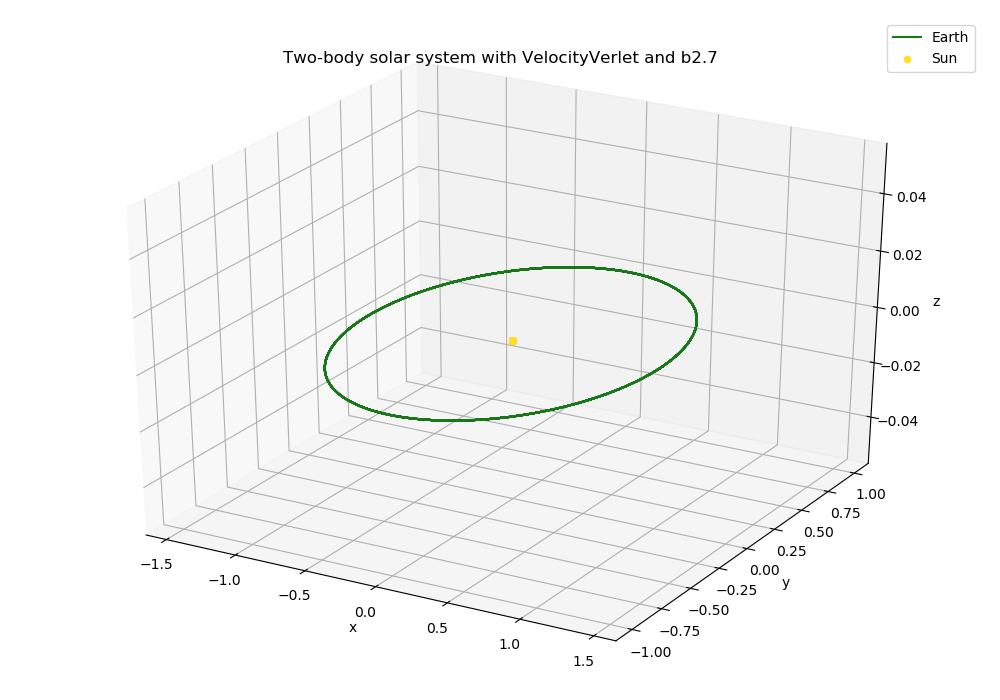
\includegraphics[width = 11cm]{img/plot3D_S_E_V_b27.png}
        \caption{Plot of the Sun-Earth solar system with $\beta = 2.7$, made with Velocity Verlet.}
        \label{fig:plot3D_S_E_V_b27}
    \end{figure}

    \begin{figure}[H]
        \centering
        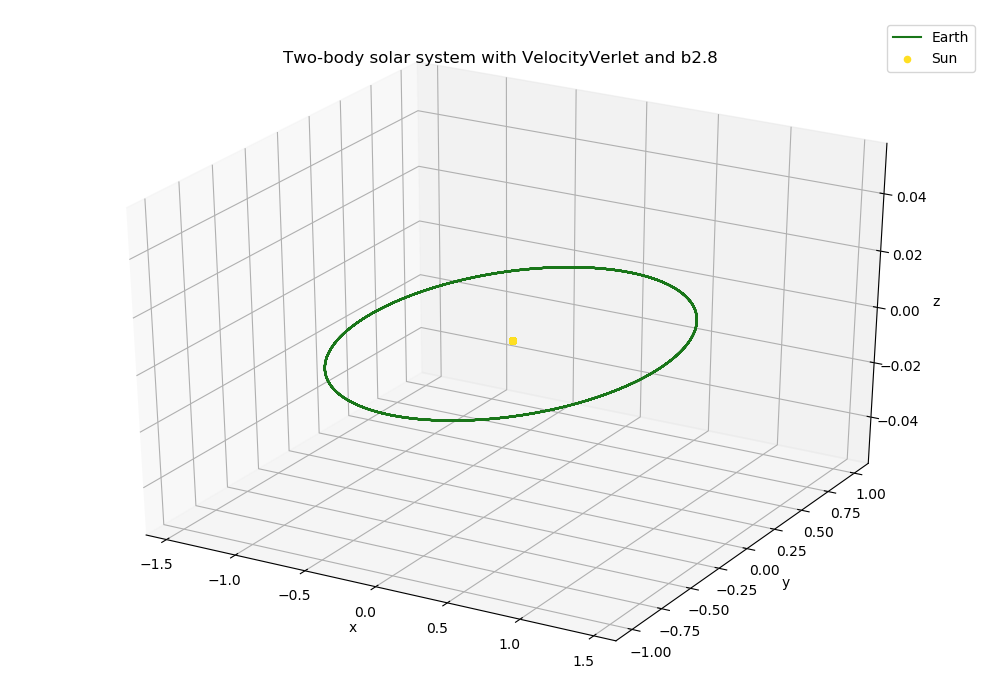
\includegraphics[width = 11cm]{img/plot3D_S_E_V_b28.png}
        \caption{Plot of the Sun-Earth solar system with $\beta = 2.8$, made with Velocity Verlet.}
        \label{fig:plot3D_S_E_V_b28}
    \end{figure}

    \begin{figure}[H]
        \centering
        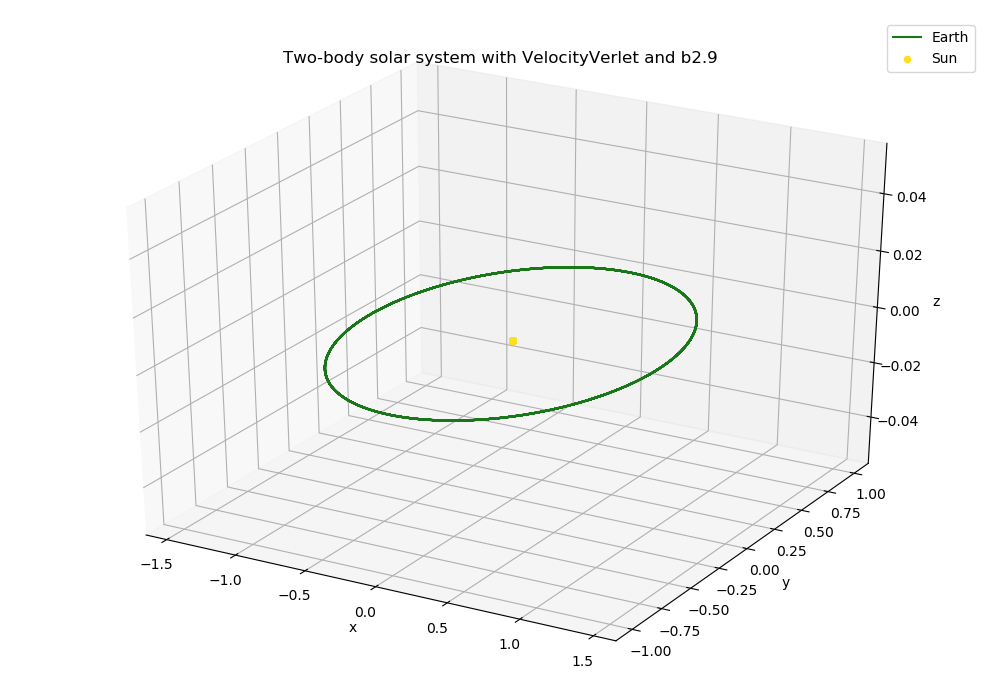
\includegraphics[width = 11cm]{img/plot3D_S_E_V_b29.png}
        \caption{Plot of the Sun-Earth solar system with $\beta = 2.9$, made with Velocity Verlet.}
        \label{fig:plot3D_S_E_V_b29}
    \end{figure}

    \begin{figure}[H]
        \centering
        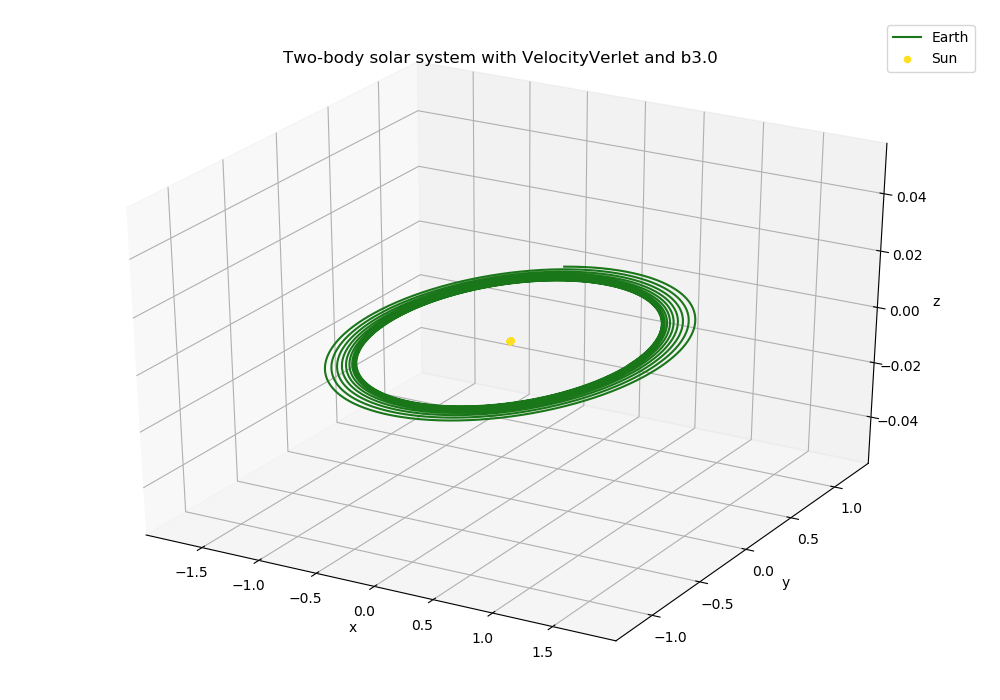
\includegraphics[width = 11cm]{img/plot3D_S_E_V_b30.png}
        \caption{Plot of the Sun-Earth solar system with $\beta = 3.0$, made with Velocity Verlet.}
        \label{fig:plot3D_S_E_V_b30}
    \end{figure}


\subsection{Sun-Mercury solar system}

    \begin{figure}[H]
        \centering
        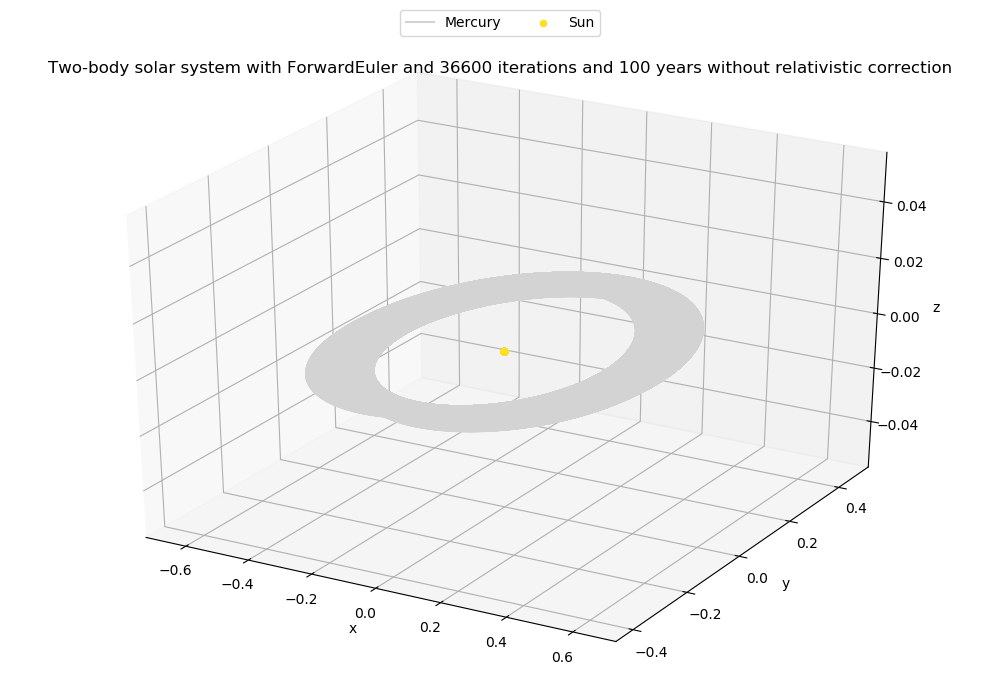
\includegraphics[width = 11cm]{img/plot3D_S_M_F_n36600_yr100_newton.png}
        \caption{Plot of the Sun-Mercury solar system with 36600 iterations over 100 years without the relativistic correction, made with Euler-Cromer.}
        \label{fig:plot3D_S_M_F_n36600_yr100_newton}
    \end{figure}

    \begin{figure}[H]
        \centering
        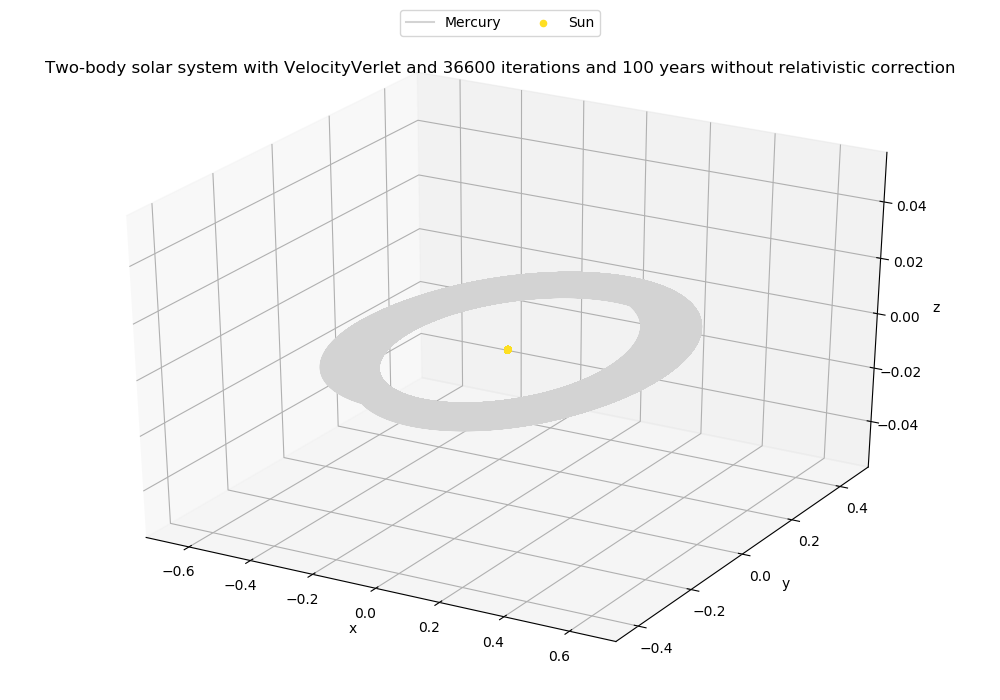
\includegraphics[width = 11cm]{img/plot3D_S_M_V_n36600_yr100_newton.png}
        \caption{Plot of the Sun-Mercury solar system with 36600 iterations over 100 years without the relativistic correction, made with Velocity Verlet.}
        \label{fig:plot3D_S_M_V_n36600_yr100_newton}
    \end{figure}

    \begin{figure}[H]
        \centering
        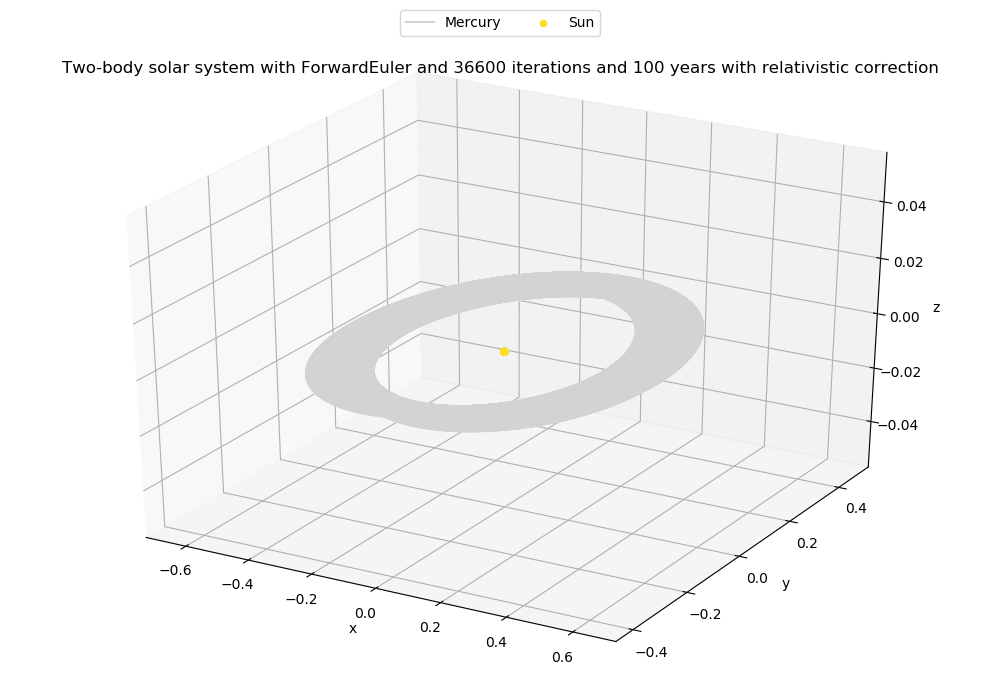
\includegraphics[width = 11cm]{img/plot3D_S_M_F_n36600_yr100.png}
        \caption{Plot of the Sun-Mercury solar system with 36600 iterations over 100 years with the relativistic correction, made with Euler-Cromer.}
        \label{fig:plot3D_S_M_F_n36600_yr100}
    \end{figure}

    \begin{figure}[H]
        \centering
        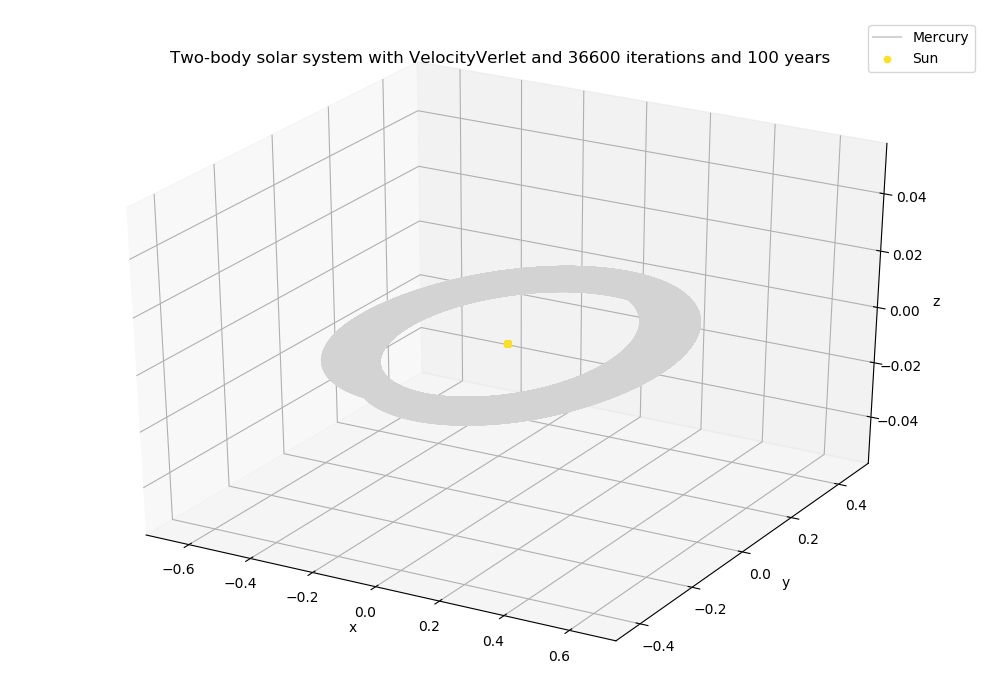
\includegraphics[width = 11cm]{img/plot3D_S_M_V_n36600_yr100.png}
        \caption{Plot of the Sun-Mercury solar system with 36600 iterations over 100 years with the relativistic correction, made with Velocity Verlet}
        \label{fig:plot3D_S_M_V_n36600_yr100}
    \end{figure}


\subsection{Sun-Earth-Jupiter solar system}

\subsubsection{Massfactor 1}

    \begin{figure}[H]
        \centering
        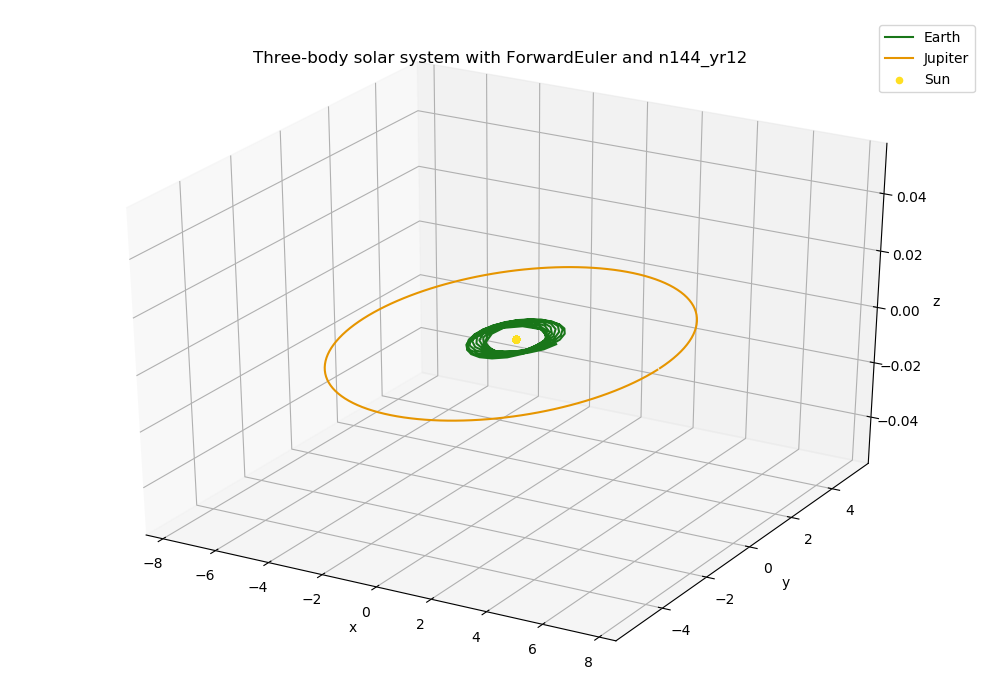
\includegraphics[width = 11cm]{img/plot3D_S_E_J_F_n144_yr12.png}
        \caption{Plot of the Sun-Earth-Jupiter solar system with 144 iterations over 12 years and a massfactor of 1 for Jupiter, made with Euler-Cromer.}
        \label{fig:plot3D_S_E_J_F_n144_yr12}
    \end{figure}

    \begin{figure}[H]
        \centering
        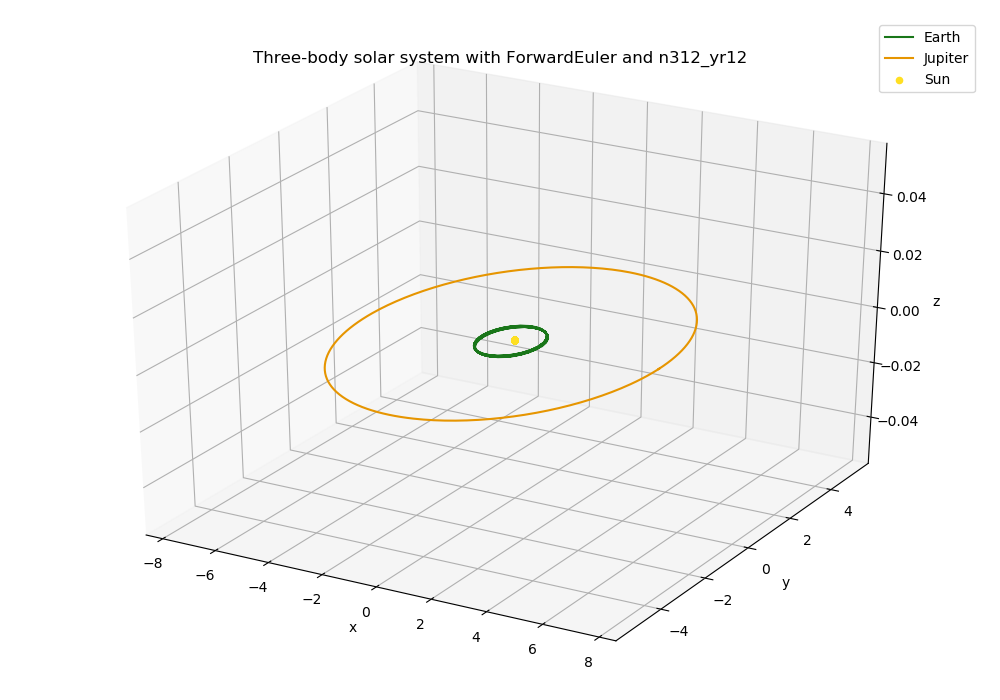
\includegraphics[width = 11cm]{img/plot3D_S_E_J_F_n312_yr12.png}
        \caption{Plot of the Sun-Earth-Jupiter solar system with 312 iterations over 12 years and a massfactor of 1 for Jupiter, made with Euler-Cromer.}
        \label{fig:plot3D_S_E_J_F_n312_yr12}
    \end{figure}

    \begin{figure}[H]
        \centering
        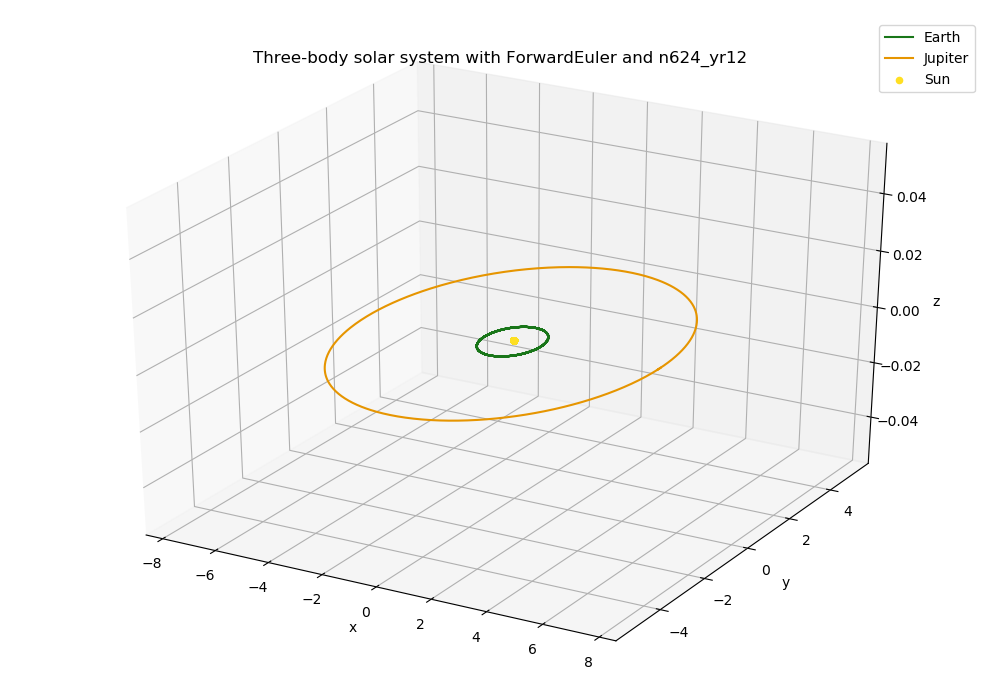
\includegraphics[width = 11cm]{img/plot3D_S_E_J_F_n624_yr12.png}
        \caption{Plot of the Sun-Earth-Jupiter solar system with 624 iterations over 12 years and a massfactor of 1 for Jupiter, made with Euler-Cromer.}
        \label{fig:plot3D_S_E_J_F_624_yr12}
    \end{figure}

    \begin{figure}[H]
        \centering
        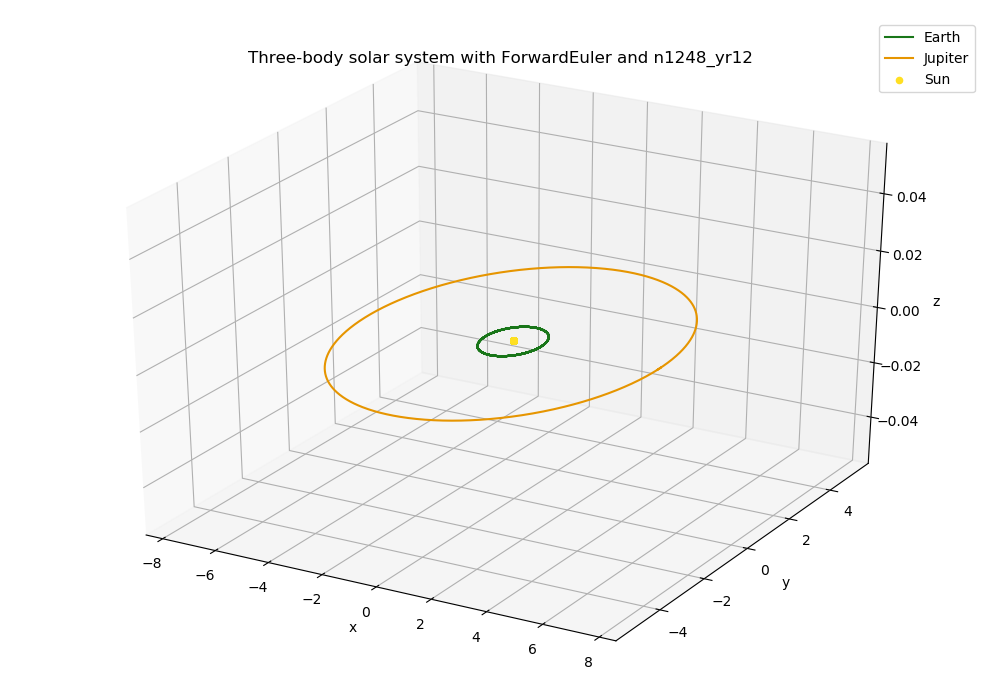
\includegraphics[width = 11cm]{img/plot3D_S_E_J_F_n1248_yr12.png}
        \caption{Plot of the Sun-Earth-Jupiter solar system with 1248 iterations over 12 years and a massfactor of 1 for Jupiter, made with Euler-Cromer.}
        \label{fig:plot3D_S_E_J_F_n1248_yr12}
    \end{figure}

    \begin{figure}[H]
        \centering
        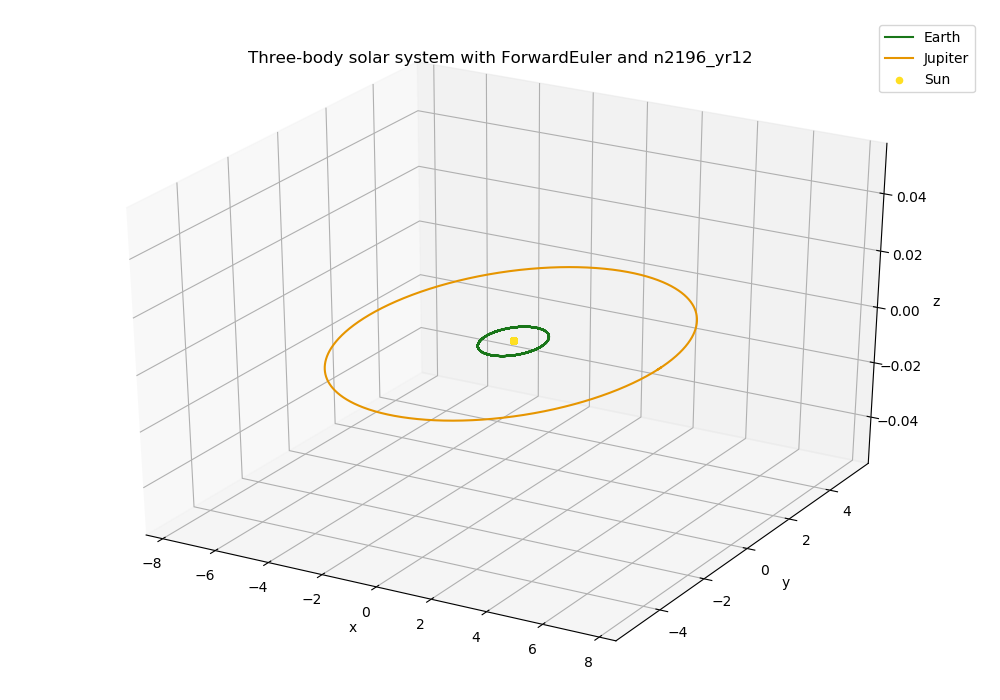
\includegraphics[width = 11cm]{img/plot3D_S_E_J_F_n2196_yr12.png}
        \caption{Plot of the Sun-Earth-Jupiter solar system with 2196 iterations over 12 years and a massfactor of 1 for Jupiter, made with Euler-Cromer.}
        \label{fig:plot3D_S_E_J_F_n2196_yr12}
    \end{figure}

    \begin{figure}[H]
        \centering
        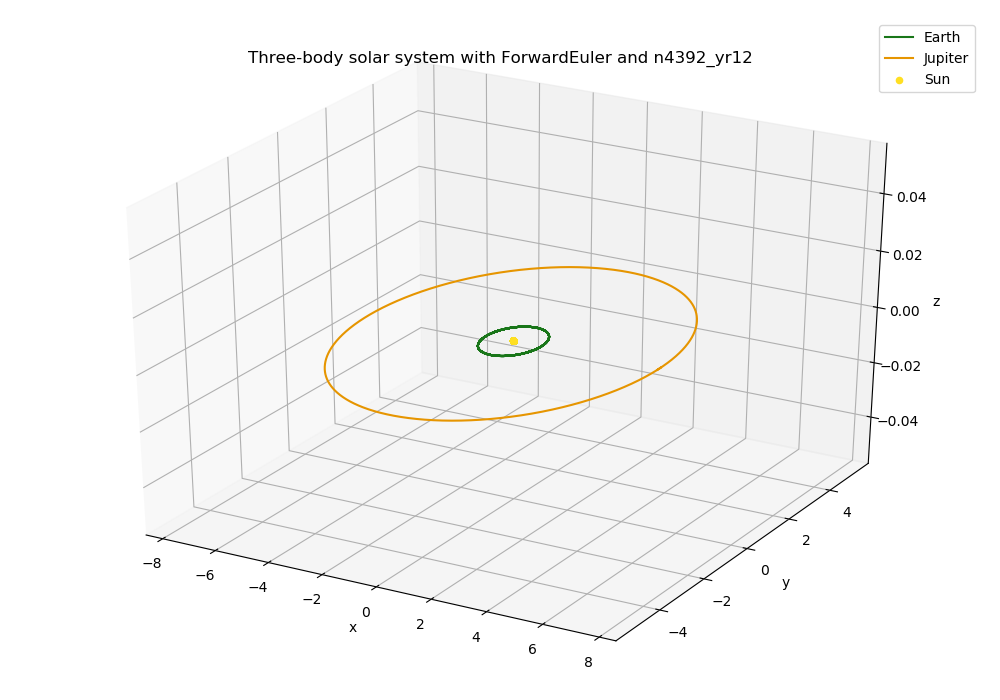
\includegraphics[width = 11cm]{img/plot3D_S_E_J_F_n4392_yr12.png}
        \caption{Plot of the Sun-Earth-Jupiter solar system with 4392 iterations over 12 years and a massfactor of 1 for Jupiter, made with Euler-Cromer.}
        \label{fig:plot3D_S_E_J_F_n4392_yr12}
    \end{figure}

    \begin{figure}[H]
        \centering
        \includegraphics[width = 11cm]{img/plot3D_S_E_J_F_n8784_yr12.png}
        \caption{Plot of the Sun-Earth-Jupiter solar system with 8784 iterations over 12 years and a massfactor of 1 for Jupiter, made with Euler-Cromer.}
        \label{fig:plot3D_S_E_J_F_n8784_yr12}
    \end{figure}

    \begin{figure}[H]
        \centering
        \includegraphics[width = 11cm]{img/plot3D_S_E_J_V_n144_yr12.png}
        \caption{Plot of the Sun-Earth-Jupiter solar system with 144 iterations over 12 years and a massfactor of 1 for Jupiter, made with Velocity Verlet.}
        \label{fig:plot3D_S_E_J_V_n144_yr12}
    \end{figure}

    \begin{figure}[H]
        \centering
        \includegraphics[width = 11cm]{img/plot3D_S_E_J_V_n312_yr12.png}
        \caption{Plot of the Sun-Earth-Jupiter solar system with 312 iterations over 12 years and a massfactor of 1 for Jupiter, made with Velocity Verlet.}
        \label{fig:plot3D_S_E_J_V_n312_yr12}
    \end{figure}

    \begin{figure}[H]
        \centering
        \includegraphics[width = 11cm]{img/plot3D_S_E_J_V_n624_yr12.png}
        \caption{Plot of the Sun-Earth-Jupiter solar system with 624 iterations over 12 years and a massfactor of 1 for Jupiter, made with Velocity Verlet.}
        \label{fig:plot3D_S_E_J_V_624_yr12}
    \end{figure}

    \begin{figure}[H]
        \centering
        \includegraphics[width = 11cm]{img/plot3D_S_E_J_V_n1248_yr12.png}
        \caption{Plot of the Sun-Earth-Jupiter solar system with 1248 iterations over 12 years and a massfactor of 1 for Jupiter, made with Velocity Verlet.}
        \label{fig:plot3D_S_E_J_V_n1248_yr12}
    \end{figure}

    \begin{figure}[H]
        \centering
        \includegraphics[width = 11cm]{img/plot3D_S_E_J_V_n2196_yr12.png}
        \caption{Plot of the Sun-Earth-Jupiter solar system with 2196 iterations over 12 years and a massfactor of 1 for Jupiter, made with Velocity Verlet.}
        \label{fig:plot3D_S_E_J_V_n2196_yr12}
    \end{figure}

    \begin{figure}[H]
        \centering
        \includegraphics[width = 11cm]{img/plot3D_S_E_J_V_n4392_yr12.png}
        \caption{Plot of the Sun-Earth-Jupiter solar system with 4392 iterations over 12 years and a massfactor of 1 for Jupiter, made with Velocity Verlet.}
        \label{fig:plot3D_S_E_J_V_n4392_yr12}
    \end{figure}

    \begin{figure}[H]
        \centering
        \includegraphics[width = 11cm]{img/plot3D_S_E_J_V_n8784_yr12.png}
        \caption{Plot of the Sun-Earth-Jupiter solar system with 8784 iterations over 12 years and a massfactor of 1 for Jupiter, made with Velocity Verlet.}
        \label{fig:plot3D_S_E_J_V_n8784_yr12}
    \end{figure}

\subsubsection{Massfactor 10}

    \begin{figure}[H]
        \centering
        \includegraphics[width = 11cm]{img/plot3D_S_E_J_F_m10_n144_yr10.png}
        \caption{Plot of the Sun-Earth-Jupiter solar system with 144 iterations over 10 years and a massfactor of 10 for Jupiter, made with Euler-Cromer.}
        \label{fig:plot3D_S_E_J_F_m10_n144_yr10}
    \end{figure}

    \begin{figure}[H]
        \centering
        \includegraphics[width = 11cm]{img/plot3D_S_E_J_F_m10_n312_yr12.png}
        \caption{Plot of the Sun-Earth-Jupiter solar system with 312 iterations over 12 years and a massfactor of 10 for Jupiter, made with Euler-Cromer.}
        \label{fig:plot3D_S_E_J_F_m10_n312_yr12}
    \end{figure}

    \begin{figure}[H]
        \centering
        \includegraphics[width = 11cm]{img/plot3D_S_E_J_F_m10_n624_yr12.png}
        \caption{Plot of the Sun-Earth-Jupiter solar system with 624 iterations over 12 years and a massfactor of 10 for Jupiter, made with Euler-Cromer.}
        \label{fig:plot3D_S_E_J_F_m10_n624_yr12}
    \end{figure}

    \begin{figure}[H]
        \centering
        \includegraphics[width = 11cm]{img/plot3D_S_E_J_F_m10_n1248_yr12.png}
        \caption{Plot of the Sun-Earth-Jupiter solar system with 1248 iterations over 12 years and a massfactor of 10 for Jupiter, made with Euler-Cromer.}
        \label{fig:plot3D_S_E_J_F_m10_n1248_yr12}
    \end{figure}

    \begin{figure}[H]
        \centering
        \includegraphics[width = 11cm]{img/plot3D_S_E_J_F_m10_n2196_yr10.png}
        \caption{Plot of the Sun-Earth-Jupiter solar system with 2196 iterations over 10 years and a massfactor of 10 for Jupiter, made with Euler-Cromer.}
        \label{fig:plot3D_S_E_J_F_m10_n2196_yr10}
    \end{figure}

    \begin{figure}[H]
        \centering
        \includegraphics[width = 11cm]{img/plot3D_S_E_J_F_m10_n4392_yr10.png}
        \caption{Plot of the Sun-Earth-Jupiter solar system with 4392 iterations over 10 years and a massfactor of 10 for Jupiter, made with Euler-Cromer.}
        \label{fig:plot3D_S_E_J_F_m10_n4392_yr10}
    \end{figure}

    \begin{figure}[H]
        \centering
        \includegraphics[width = 11cm]{img/plot3D_S_E_J_F_m10_n8784_yr12.png}
        \caption{Plot of the Sun-Earth-Jupiter solar system with 8784 iterations over 12 years and a massfactor of 10 for Jupiter, made with Euler-Cromer.}
        \label{fig:plot3D_S_E_J_F_m10_n8784_yr12}
    \end{figure}

    \begin{figure}[H]
        \centering
        \includegraphics[width = 11cm]{img/plot3D_S_E_J_V_m10_n144_yr10.png}
        \caption{Plot of the Sun-Earth-Jupiter solar system with 144 iterations over 10 years and a massfactor of 10 for Jupiter, made with Velocity Verlet.}
        \label{fig:plot3D_S_E_J_V_m10_n144_yr10}
    \end{figure}

    \begin{figure}[H]
        \centering
        \includegraphics[width = 11cm]{img/plot3D_S_E_J_V_m10_n312_yr12.png}
        \caption{Plot of the Sun-Earth-Jupiter solar system with 312 iterations over 12 years and a massfactor of 10 for Jupiter, made with Velocity Verlet.}
        \label{fig:plot3D_S_E_J_V_m10_n312_yr12}
    \end{figure}

    \begin{figure}[H]
        \centering
        \includegraphics[width = 11cm]{img/plot3D_S_E_J_V_m10_n624_yr12.png}
        \caption{Plot of the Sun-Earth-Jupiter solar system with 624 iterations over 12 years and a massfactor of 10 for Jupiter, made with Velocity Verlet.}
        \label{fig:plot3D_S_E_J_V_m10_n624_yr12}
    \end{figure}

    \begin{figure}[H]
        \centering
        \includegraphics[width = 11cm]{img/plot3D_S_E_J_V_m10_n1248_yr12.png}
        \caption{Plot of the Sun-Earth-Jupiter solar system with 1248 iterations over 12 years and a massfactor of 10 for Jupiter, made with Velocity Verlet.}
        \label{fig:plot3D_S_E_J_V_m10_n1248_yr12}
    \end{figure}

    \begin{figure}[H]
        \centering
        \includegraphics[width = 11cm]{img/plot3D_S_E_J_V_m10_n2196_yr10.png}
        \caption{Plot of the Sun-Earth-Jupiter solar system with 2196 iterations over 10 years and a massfactor of 10 for Jupiter, made with Velocity Verlet.}
        \label{fig:plot3D_S_E_J_V_m10_n2196_yr10}
    \end{figure}

    \begin{figure}[H]
        \centering
        \includegraphics[width = 11cm]{img/plot3D_S_E_J_V_m10_n4392_yr10.png}
        \caption{Plot of the Sun-Earth-Jupiter solar system with 4392 iterations over 10 years and a massfactor of 10 for Jupiter, made with Velocity Verlet.}
        \label{fig:plot3D_S_E_J_V_m10_n4392_yr10}
    \end{figure}

    \begin{figure}[H]
        \centering
        \includegraphics[width = 11cm]{img/plot3D_S_E_J_V_m10_n8784_yr12.png}
        \caption{Plot of the Sun-Earth-Jupiter solar system with 8784 iterations over 12 years and a massfactor of 10 for Jupiter, made with Velocity Verlet.}
        \label{fig:plot3D_S_E_J_V_m10_n8784_yr12}
    \end{figure}

\subsubsection{Massfactor 1000}

    \begin{figure}[H]
        \centering
        \includegraphics[width = 11cm]{img/plot3D_S_E_J_F_m1000_n144_yr12.png}
        \caption{Plot of the Sun-Earth-Jupiter solar system with 144 iterations over 12 years and a massfactor of 1000 for Jupiter, made with Euler-Cromer.}
        \label{fig:plot3D_S_E_J_F_m1000_n144_yr12}
    \end{figure}

    \begin{figure}[H]
        \centering
        \includegraphics[width = 11cm]{img/plot3D_S_E_J_F_m1000_n312_yr12.png}
        \caption{Plot of the Sun-Earth-Jupiter solar system with 312 iterations over 12 years and a massfactor of 1000 for Jupiter, made with Euler-Cromer.}
        \label{fig:plot3D_S_E_J_F_m1000_n312_yr12}
    \end{figure}

    \begin{figure}[H]
        \centering
        \includegraphics[width = 11cm]{img/plot3D_S_E_J_F_m1000_n624_yr12.png}
        \caption{Plot of the Sun-Earth-Jupiter solar system with 624 iterations over 12 years and a massfactor of 1000 for Jupiter, made with Euler-Cromer.}
        \label{fig:plot3D_S_E_J_F_m1000_n624_yr12}
    \end{figure}

    \begin{figure}[H]
        \centering
        \includegraphics[width = 11cm]{img/plot3D_S_E_J_F_m1000_n1248_yr12.png}
        \caption{Plot of the Sun-Earth-Jupiter solar system with 1248 iterations over 12 years and a massfactor of 1000 for Jupiter, made with Euler-Cromer.}
        \label{fig:plot3D_S_E_J_F_m1000_n1248_yr12}
    \end{figure}

    \begin{figure}[H]
        \centering
        \includegraphics[width = 11cm]{img/plot3D_S_E_J_F_m1000_n2196_yr12.png}
        \caption{Plot of the Sun-Earth-Jupiter solar system with 2196 iterations over 12 years and a massfactor of 1000 for Jupiter, made with Euler-Cromer.}
        \label{fig:plot3D_S_E_J_F_m1000_n2196_yr12}
    \end{figure}

    \begin{figure}[H]
        \centering
        \includegraphics[width = 11cm]{img/plot3D_S_E_J_F_m1000_n4392_yr12.png}
        \caption{Plot of the Sun-Earth-Jupiter solar system with 4392 iterations over 12 years and a massfactor of 1000 for Jupiter, made with Euler-Cromer.}
        \label{fig:plot3D_S_E_J_F_m1000_n4392_yr12}
    \end{figure}

    \begin{figure}[H]
        \centering
        \includegraphics[width = 11cm]{img/plot3D_S_E_J_F_m1000_n8784_yr12.png}
        \caption{Plot of the Sun-Earth-Jupiter solar system with 8784 iterations over 12 years and a massfactor of 1000 for Jupiter, made with Euler-Cromer.}
        \label{fig:plot3D_S_E_J_F_m1000_n8784_yr12}
    \end{figure}

    \begin{figure}[H]
        \centering
        \includegraphics[width = 11cm]{img/plot3D_S_E_J_V_m1000_n144_yr12.png}
        \caption{Plot of the Sun-Earth-Jupiter solar system with 144 iterations over 12 years and a massfactor of 1000 for Jupiter, made with Velocity Verlet.}
        \label{fig:plot3D_S_E_J_V_m1000_n144_yr12}
    \end{figure}

    \begin{figure}[H]
        \centering
        \includegraphics[width = 11cm]{img/plot3D_S_E_J_V_m1000_n312_yr12.png}
        \caption{Plot of the Sun-Earth-Jupiter solar system with 312 iterations over 12 years and a massfactor of 1000 for Jupiter, made with Velocity Verlet.}
        \label{fig:plot3D_S_E_J_V_m1000_n312_yr12}
    \end{figure}

    \begin{figure}[H]
        \centering
        \includegraphics[width = 11cm]{img/plot3D_S_E_J_V_m1000_n624_yr12.png}
        \caption{Plot of the Sun-Earth-Jupiter solar system with 624 iterations over 12 years and a massfactor of 1000 for Jupiter, made with Velocity Verlet.}
        \label{fig:plot3D_S_E_J_V_m1000_n624_yr12}
    \end{figure}

    \begin{figure}[H]
        \centering
        \includegraphics[width = 11cm]{img/plot3D_S_E_J_V_m1000_n1248_yr12.png}
        \caption{Plot of the Sun-Earth-Jupiter solar system with 1248 iterations over 12 years and a massfactor of 1000 for Jupiter, made with Velocity Verlet.}
        \label{fig:plot3D_S_E_J_V_m1000_n1248_yr12}
    \end{figure}

    \begin{figure}[H]
        \centering
        \includegraphics[width = 11cm]{img/plot3D_S_E_J_V_m1000_n2196_yr12.png}
        \caption{Plot of the Sun-Earth-Jupiter solar system with 2196 iterations over 12 years and a massfactor of 1000 for Jupiter, made with Velocity Verlet.}
        \label{fig:plot3D_S_E_J_V_m1000_n2196_yr12}
    \end{figure}

    \begin{figure}[H]
        \centering
        \includegraphics[width = 11cm]{img/plot3D_S_E_J_V_m1000_n4392_yr12.png}
        \caption{Plot of the Sun-Earth-Jupiter solar system with 4392 iterations over 12 years and a massfactor of 1000 for Jupiter, made with Velocity Verlet.}
        \label{fig:plot3D_S_E_J_V_m1000_n4392_yr12}
    \end{figure}

    \begin{figure}[H]
        \centering
        \includegraphics[width = 11cm]{img/plot3D_S_E_J_V_m1000_n8784_yr12.png}
        \caption{Plot of the Sun-Earth-Jupiter solar system with 8784 iterations over 12 years and a massfactor of 1000 for Jupiter, made with Velocity Verlet.}
        \label{fig:plot3D_S_E_J_V_m1000_n8784_yr12}
    \end{figure}

\subsection{Dynamic sun}

    \begin{figure}[H]
        \centering
        \includegraphics[width = 11cm]{img/plot3D_S_E_J_F_dynamic_sun.png}
        \caption{Plot of the Sun-Earth-Jupiter solar system with a dynamic sun, made with Euler-Cromer.}
        \label{fig:plot3D_S_E_J_F_dynamic_sun}
    \end{figure}

    \begin{figure}[H]
        \centering
        \includegraphics[width = 11cm]{img/plot3D_S_E_J_V_dynamic_sun.png}
        \caption{Plot of the Sun-Earth-Jupiter solar system with a dynamic sun, made with Velocity Verlet.}
        \label{fig:plot3D_S_E_J_V_dynamic_sun}
    \end{figure}


\subsection{Ten-body solar system}

\subsubsection{Static sun}

    \begin{figure}[H]
        \centering
        \includegraphics[width = 11cm]{img/plot3D_10body_F_n3660_yr10.png}
        \caption{Plot of the ten-body solar system with 3660 iterations over 10 years with a static sun, made with Euler-Cromer.}
        \label{fig:plot3D_10body_F_n3660_yr10}
    \end{figure}

    \begin{figure}[H]
        \centering
        \includegraphics[width = 11cm]{img/plot3D_10body_V_n3660_yr10.png}
        \caption{Plot of the ten-body solar system with 3660 iterations over 10 years with a static sun, made with Velocity Verlet.}
        \label{fig:plot3D_10body_V_n3660_yr10}
    \end{figure}

\subsubsection{Dynamic sun}

    \begin{figure}[H]
        \centering
        \includegraphics[width = 11cm]{img/plot3D_10body_F_n3660_yr10_dynamic_sun.png}
        \caption{Plot of the ten-body solar system with 3660 iterations over 10 years with a dynamic sun, made with Euler-Cromer.}
        \label{fig:plot3D_10body_F_n3660_yr10_dynamic_sun}
    \end{figure}

    \begin{figure}[H]
        \centering
        \includegraphics[width = 11cm]{img/plot3D_10body_V_n3660_yr10_dynamic_sun.png}
        \caption{Plot of the ten-body solar system with 3660 iterations over 10 years with a dynamic sun, made with Velocity Verlet.}
        \label{fig:plot3D_10body_V_n3660_yr10_dynamic_sun}
    \end{figure}


%--------------- Discussion ---------------------------------------
\vspace{1cm}

\clearpage
\newpage

\section{Discussion} \label{sec:Discussion}


\subsection{Stability of the Sun-Earth solar system given by the Euler-Cromer method and the Velocity Verlet method}    \label{sec:stabilitySE}

    Figures (\ref{fig:plot3D_S_E_F_n120_yr10}) through (\ref{fig:plot3D_S_E_V_n520_yr10}) plots the Sun-Earth solar system for different iterations. Here it is possible to see that an increasing number of iterations will improve the stability of Earth's orbit around the Sun.
    For figure (\ref{fig:plot3D_S_E_F_n120_yr10}) and (\ref{fig:plot3D_S_E_V_n120_yr10}) the Earth's orbit is not stable, given by that the orbit changes position drastically. The Velocity Verlet method demonstrates how it is a better approximation than Euler-Cromer given by that the orbit changes less and is therefore more stable. By increasing the number of iterations to $n = 260$ the orbit has stabilized by a lot for both methods, though mostly for Velocity Verlet which is almost indistinguishable from the next iteration step with $n = 520$. With further increase to $n = 520$ both methods have stabilized compared to a higher number of iterations.
    Figures (\ref{fig:plot3D_S_E_F_n520_yr10}) and (\ref{fig:plot3D_S_E_V_n520_yr10}) illustrates this. The plot given by the Euler-Cromer method may have a small increase in stability by a higher number of iterations, but given by the figures for the Velocity Verlet method this should be very small. Originally this test of the two methods have data for other larger numbers of iterations, but seeing as the orbits have seemingly stabilized we deemed the plotting of these datas as unnecessary.
    The stability should increase by an increasing number of iterations because a larger number of iterations means that more changes in the bodies in the solar system can be accounted for, giving a more accurate representation of the solar system. The stabilizing of the Earth's orbit therefore implies the stability of the Euler-Cromer method and the Velocity Verlet method. \\

    The number of FLOPs for one iterations is for Euler-Cromer $(2n + 8)_\gamma + 4$ and for Velocity Verlet $(2n + 8)_\gamma + 6$, where $n$ is the number of iterations and $\gamma$ is the number of planets. Therefore, the Velocity Verlet should use longer time to compute, because it has more operations to compute. The timings is listed in the table (\ref{tab:timings}) and supports the theory of FLOPs. The table shows that Euler-Cromer used 26 s whereas Velocity Verlet used 34 s. Euler-Cromer used fewer seconds because it had fewer FLOPs. However, the approximation of Velocity Verlet is better than Euler-Cromer, hence the time difference is easy to overlook to instead have better accuracy of the solar system. When looking at all iterations performed, the FLOPs above should be multiplied with $n$ for the number of iterations. \\

    When looking at the conservation of energy for the two different methods, it is possible to see that Euler-Cromer does not conserve energy, whereas Velocity Verlet does. This is because plots of the Sun-Earth system with Euler-Cromer has an orbit of the Earth which moves around the Sun, while the orbit for the Earth with Velocity Verlet just rotates around the Sun. Figures (\ref{fig:plot3D_S_E_F_n120_yr10}) and (\ref{fig:plot3D_S_E_V_n120_yr10}) illustrates this the best. The conservation of energy is important in simulations of the solar system because energy has an important effect on the orbit of the planets. This is shown by the plots with the Velocity Verlet method, which conserves energy, and how the orbits are rounder and more consistent. \\


\subsection{The escape velocity of the Earth in the Sun-Earth solar system} \label{sec:escapevelocitySE}

    The plots of the escape velocity is given in figures (\ref{fig:plot3D_S_E_V_vel100pi}) through (\ref{fig:plot3D_S_E_V_vel300pi}).
    From the theory and appendix, equation (\ref{eq:theoretical escapevelocity}) and section \ref{sec:escapevelocity}, the theoretical escape velocity of the Earth is $v_p = 8.886$ m/s, which is a little smaller than $2.8 \pi$. Therefore, it is expected that the Earth will not escape its orbit around the Sun until the initial velocity of the planet is around $2.8 \pi$.
    In figure (\ref{fig:plot3D_S_E_V_vel100pi}) the Earth keeps its orbit, which is expected as the velocity is $1.0 \pi$.
    The same applies for figures (\ref{fig:plot3D_S_E_V_vel200pi}) and (\ref{fig:plot3D_S_E_V_vel250pi}), with respectively an initial velocity of $2.0 \pi$ and $2.5 \pi$.
    For figure (\ref{fig:plot3D_S_E_V_vel275pi}) it is possible to see that Earth escapes. This is not in agreement with the theoretical escape velocity.
    However, around $x = -15$ Earth starts to move back to the Sun. The Earth does not escape successfully, and with more iterations, which gives more positions, the Earth should return to its orbit around the Sun. For figure (\ref{fig:plot3D_S_E_V_vel280pi}), with an initial velocity of $2.8 \pi$, the Earth has successfully escaped, as expected from the theoretical escape velocity. Figure (\ref{fig:plot3D_S_E_V_vel300pi}) further illustrates the escape with initial velocity over the theoretical escape velocity, where the initial velocity is $3.0 \pi$. \\

\subsection{Varying \texorpdfstring{$\beta$}{TEXT} for the Sun-Earth solar system}    \label{sec:betaSE}

    The plots of the varying of $\beta$ is given in figures (\ref{fig:plot3D_S_E_V_b20}) through (\ref{fig:plot3D_S_E_V_b30}). $\beta$ is the number which denotes the exponent of the distance between the Earth and the Sun, given in the equation (\ref{eq:gravitationalforce}) below.

    \begin{equation}    \label{eq:gravitationalforce}
        F_G = \frac{G M_\odot M_{earth}}{r^\beta}
    \end{equation} \\

    By increasing the value of $\beta$ the gravitational force should become smaller. This means that the Sun should have less effect on the orbit of the Earth, and the Earth could possibly escape the solar system. When $\beta = 2$, which gives the regular gravitational force when substituted in equation (\ref{eq:gravitationalforce}, the Earth behaves as normal. Figure (\ref{fig:plot3D_S_E_V_b20}) shows this. With increasing $\beta$ from 2.0 to 2.9 there is no apparent visible difference. However, when $\beta = 3.0$ the Earth slowly goes in a larger orbit around the Sun. This means that the gravitational force which holds Earth in its orbit is too small, and the Earth escapes. This is seen in figure (\ref{fig:plot3D_S_E_V_b30}). \\

\subsection{Stability of the Sun-Earth-Jupiter solar system}    \label{sec:stabilitySEJ}

    As the program went from Sun-Earth to Sun-Earth-Jupiter it was interesting to watch how the system would change, and to see how the program handled a three-body problem. Looking at figure (\ref{fig:plot3D_S_E_J_F_n4392_yr12}) and (\ref{fig:plot3D_S_E_J_V_n4392_yr12}) we can see that Euler and Verlet is more or less the same.\\

    Looking at stability one can see that the system looks pretty stable already at $n=312$ and $yr=12$ (measure every other week). The system looks really stable and has visually no difference after $n=1248$ (measure twice per week). To see more about the measuring frequencies, look at section (\ref{sec:frequencies}).\\

\subsection{Varying mass for Jupiter in the Sun-Earth-Jupiter solar system} \label{sec:massSEJ}

    For the normal mass of Jupiter, it can bee seen that the movement of Earth does not change noticeably from the Sun-Earth case. Looking at the case where Jupiter is 10x as heavy there does not \underline{seem} to be a difference, and when Jupiter is 1000x as heavy the orbit just seems thicker.\\

    Looking at the gifs for these runs the differences is much more noticeable. \href{https://github.com/Erikbgram/Fys3150/blob/master/Project\%205/img/ani3D_S_E_J_V_n144_yr12.gif}{Normal mass of Jupiter}, \href{https://github.com/Erikbgram/Fys3150/blob/master/Project\%205/img/ani3D_S_E_J_V_m10_n144_yr12.gif}{10x mass of Jupiter} and \href{https://github.com/Erikbgram/Fys3150/blob/master/Project\%205/img/ani3D_S_E_J_V_m1000_n144_yr12.gif}{10x mass of Jupiter}.
    Though these gifs have a low iteration-count it is easy to see how Jupiter slighly pulls the orbit of the Earth towards the position of Jupiter. For larger masses this is much more noticeable.

\subsection{Moving Sun in the in the Sun-Earth-Jupiter solar system}

    For Velocity Verlet the Sun spirals of out of the solar system. See figure (\ref{fig:plot3D_S_E_J_V_n4392_yr12}). It might be that there was too few iterations, and so something went wrong. At the same time, since Velocity Verlet conserves energy, it should not happen. This could mean there is an error in the program that has gone unnoticed.\\

    Looking at The Euler-Cromer method the Sun stays in a stable orbit. See figure (\ref{fig:plot3D_S_E_J_F_n4392_yr12}). Jupiter's orbit stars going skew. The static Sun-case simulated everything in the xy-plane, whilst the dynamic Sun-case took NASA's data \cite{solarsystemdata}. It could be that the real data has a more skew motion of the planets' orbits. Nevertheless, the data ssems to show a stable system. This is good, and an indication that a static sun is a good approximation. Most likely, had the static Sun-simulation used real data, the orbit would be more or less identical to the ones in the system with a dynamic Sun.

\subsection{Model for all planets of the solar system}      \label{sec:tenbody}

    Extend your program to include all planets in the solar system (if you
    have time, you can also include the various moons, but it is not required) and
    discuss your results.

    Figures (\ref{fig:plot3D_10body_F_n3660_yr10})-(\ref{fig:plot3D_10body_V_n3660_yr10_dynamic_sun}) shows the plots of the complete solar system. One interesting thing to note right off the bat is that for system with a dynamic sun, the Velocity Verlet algorithm makes Venus slingshot out into outer space. A possible reason for this can be to few iterations. Looking closer and trying with $n=7320$, Venus flew off faster and longer. $n=7320$ and $yr=10$ would be two measuring points per day. One would think this was enough iterations for the problem to disappear, yet it did not. It might be that the problem disapeared if we had ran even more iterations. This seems very strange considering the fact that Velocity Verlet has worked flawlessly for all other runs and that the data is fetched from NASA \cite{solarsystemdata}. This does not happen when using a static sun.\\

    When comparing the Euler-Cromer plots for static, figure (\ref{fig:plot3D_10body_F_n3660_yr10}), and dynamic sun, figure (\ref{fig:plot3D_10body_F_n3660_yr10_dynamic_sun}), it is possible to see that there is practically no difference. This is excellent and means that a static Sun is a good approximation for the solar system! It is quite interesting to see how the solar system evolves over ten years. For the inner solar system (Mercury to Mars) the bodies completes a full revolution, or more, around the Sun. Looking at the outer solar system (Jovian planets + Pluto) a full revolution is not reached. This is due to the immense distance they have to travel, and the velocity they have. Had the simulation been for $\approx250$ years we would see even Pluto complete it's revolution as its orbital period is $\approx 248$ years.

\subsection{Perihelion precession of Mercury}

    Looking at the perihelion precession of Mercury an iteration-count of 36600 was used over 100 years, as this was more than enough for all other runs. The data is shown in figure (\ref{fig:plot3D_S_M_V_n36600_yr100_newton}) and (\ref{fig:plot3D_S_M_V_n36600_yr100}). The 1st of the two is using non-relativistic gravity, whilst the 2nd is with relativistic gravity. The difference in the plots is not noticeable, which means that the relativistic correction might have been incorrect. The likeness can also be attributed to the fact that the amount of iterations was too low. Having looked around a bit, it seemed other people doing the same simulations had used a lot more iterations (around $10^8$ or more).\\

    Evaluating the data in \href{https://github.com/Erikbgram/Fys3150/blob/master/Project\%205/program/perihelion.py}{perihelion.py} one can see that something is quite wrong. This could be from a faulty conversion from radians to arc-seconds, or to the crude method of picking out data-points. Nevertheless, the last value (which should be 43 arc-seconds) turns out to be $\approx-195000$ which is WAY too much. Even in radians the value is $\approx-0.942$, even though it should be multiple magnitudes lower.\\

    Sadly there was not enough time to bug fix the issue. However, the issue was looked into and attempted to be solved. It can be assumed that the relativistic addition to the equation of gravitional force made a better prediction of the perihelion precession of Mercury.

%---------------Conclusion and perspective---------------------------
\vspace{1cm}

\section{Conclusion and perspective} \label{sec:Conclusion}

\iffalse
Conclusions and perspectives

What should I focus on? Conclusions.
State your main findings and interpretations
Try as far as possible to present perspectives for future work
Try to discuss the pros and cons of the methods and possible improvements \\
\fi

    In this numerical study the solar system was simulated with two different numerical methods. The solar systems studied was the Sun-Earth solar system, the Sun-Mercury solar system, the Sun-Earth-Jupiter solar system and the whole ten-body solar system including the dwarf planet Pluto. The two methods used were Euler-Cromer, which does not conserve energy, and Velocity Verlet, which conserves energy. Conservation of energy proved to have an important effect on the stability of the solar systems. See sections (\ref{sec:stabilitySE}) and (\ref{sec:stabilitySEJ}) for the discussion of the stability of the Sun-Earth solar system and the Sun-Earth-Jupiter solar system. Here the superiourness of the Velocity Verlet was proven, even though it used a longer computation time. For the Sun-Earth solar system we tested the escape velocity of Earth in comparison to the theoretical value calculated in the appendix, see section \ref{sec:escapevelocity} and equation (\ref{eq:theoretical escapevelocity}). The discussion is in the section \ref{sec:escapevelocitySE}. Here it was found that the escape velocity from our data is almost exactly that of the theoretical. Further for the Sun-Earth solar system we tested the gravitational force from the Sun on the Earth with differing exponents of the distance between the two objects, see section \ref{sec:betaSE}. This also behaved as expected. When looking at the Sun-Earth-Jupiter we can see that increasing the mass of Jupiter by factors of 1, 10 and 1000 with differing number of iterations, will affect Earth's orbit in the solar system, see section \ref{sec:massSEJ}. For the ten-body solar system it is interesting to see how vastly different the distances between the planets to the Sun are and their orbital velocity. This is most visible by the fact that most planets does not make a full revolution around the Sun by ten years. See the section \ref{sec:tenbody}. This study has in conclusion shown the difference between the two numerical methods by their simulation of the solar system, and given interesting and cool simulations of the solar system.


%----------------References----------------------------------------

\vspace{1cm}

\section{References} \label{sec:References}

\iffalse
What should I focus on? References.
Give always references to material you base your work on, either scientific articles/reports or books.
Refer to articles as: name(s) of author(s), journal, volume (boldfaced), page and year in parenthesis.
Refer to books as: name(s) of author(s), title of book, publisher, place and year, eventual page numbers
\fi

\begin{thebibliography}{}

\bibitem{task}
Morten H. Jensen (2019), \href{https://github.com/CompPhysics/ComputationalPhysics/blob/master/doc/Projects/2019/Project5/SolarSystem/pdf/SolarSystem.pdf}{Project 5}, Departement of Physics, University of Oslo, Norway

\bibitem{github}
Erik B. Grammeltvedt, Alexandra Jahr Kolstad, Erlend T. North (2019), \href{https://github.com/Erikbgram/Fys3150}{GitHub}, Students of Departement of Physics, University of Oslo, Norway

\bibitem{lecture_slides}
Morten H. Jensen (2015), \href{https://github.com/CompPhysics/ComputationalPhysics/blob/master/doc/Lectures/lectures2015.pdf}{Lecture slides for FYS3150}, Department of Physics, University of Oslo, Norway

\bibitem{solarsystemdata}
Jon. D. Giorgini (2019), \href{https://ssd.jpl.nasa.gov/horizons.cgi#top}{Physical data of the planets and the sun.}, Solar System Dynamics Group, Horizons On-Line Ephemeris System, Jet Propulsion Laboratory, Pasadena, California, USA

\end{thebibliography}


%--------------Appendix---------------------------------------------
\vspace{1cm}


\appendix
\section{Appendix} \label{sec:Appendix}

\iffalse
Appendix with extra material

What should I focus on? additional material.
Additional calculations used to validate the codes
Selected calculations, these can be listed with few comments
Listing of the code if you feel this is necessary
You can consider moving parts of the material from the methods section to the appendix. You can also place additional material on your webpage.

\fi

\subsection{Mass-conversion} \label{app:mass}

    \begin{table}[H]
        \centering
        \caption{Astronomical data retrieved from \cite{solarsystemdata}. }
        \vspace{2mm}
        \label{tab:mass}
        \begin{tabular}{|c|c|c|c|}
            \hline
            Celestial Body & Mass [kg] & Mass [$M_{\odot}$] & Distance to sun [AU]\\
            \hline \hline
            Sun     & $ 2    \cdot10^{30} $ & 1                    & 0 \\
            Mercury & $ 3.3  \cdot10^{23} $ & $1.65 \cdot 10^{-7}$ & 0.39 \\
            Venus   & $ 4.9  \cdot10^{24} $ & $2.45 \cdot 10^{-6}$ & 0.72 \\
            Earth   & $ 6    \cdot10^{24} $ & $3.0 \cdot 10^{-6}$  & 1 \\
            Mars    & $ 6.6  \cdot10^{23} $ & $3.3 \cdot 10^{-7}$  & 1.52 \\
            Jupiter & $ 1.9  \cdot10^{27} $ & $9.5 \cdot 10^{-4}$  & 5.20 \\
            Saturn  & $ 5.5  \cdot10^{26} $ & $2.75 \cdot 10^{-4}$ & 9.54 \\
            Uranus  & $ 8.8  \cdot10^{25} $ & $4.4 \cdot 10^{-5}$  & 19.19 \\
            Neptune & $ 1.03 \cdot10^{26} $ & $5.15 \cdot 10^{-5}$ & 30.06 \\
            Pluto   & $ 1.31 \cdot10^{22} $ & $6.55 \cdot 10^{-9}$ & 39.53 \\
            \hline
        \end{tabular} \\
        \hspace{0pt}\\
    \end{table}

\subsection{Explaining the calculation of a planets escape velocity} \label{sec:escapevelocity}

    As some of these problems are solvable by hand there are some calculations that can be done prior to the simulations in order to have something to compare results with. For instance one can quite easily calculate a planets escape velocity from the Sun. One can use that the escape velocity would be the lowest energy required to move the planet out of the gravitational pool from the Sun. In that case the planet would be left with zero kinetic energy. Because the planet is moved out of the gravitational field the potential energy would also bee 0. Therefore the expression for the system will be given as equation (\ref{eq:U=K}). This is with the condition that there is no other forces acting on the system except for the gravitational force.   \\

    \begin{equation}    \label{eq:U=K}
        U_i + K_i = U_f + K_f \\
    \end{equation} \\

    Due to the criteria we have set for the model and the need for conservation of energy the expression becomes: \\

    \begin{equation}    \label{eq:Kwithfinalas0}
        U_i + K_i = 0 + 0 \\
    \end{equation} \\

    The potential energy is given by the gravitational potential which is:\\

    \begin{equation}    \label{eq:gravitationalpotential}
        U = - \frac{GMm}{r} \\
    \end{equation} \\

    The kinetic energy is given by the planets kinetic energy: \\

    \begin{equation}    \label{eq:kineticpotential}
        K = \frac{1}{2} mv_p \\
    \end{equation} \\

    Therefore the escape velocity can be calculated as the kinetic energy being equal to the potential energy. \\

    \begin{equation} \label{eq:escapevelocity}
        v_p =  \sqrt{\frac{2GM}{r}}
    \end{equation} \\

\subsection{Rewriting Newtons second law of motion} \label{sec:n2l}

    Newtons second law of motion is stated in equation (\ref{eq:n2l}).

    \begin{equation} \label{eq:n2l}
        F = ma \\
    \end{equation} \\

    Equation (\ref{eq:n2l}) can be written as a differential equation that will give the force as a function of position (\ref{eq:diffn2l}).\\

    \begin{equation}    \label{eq:diffn2l}
        F(x,t) = m\frac{d^{2}x}{dt^{2}}\\
    \end{equation} \\

    Since we know that the velocity, $v$, is given as a function of change in position over change in time. This gives us equation (\ref{eq:diffvelocity}).\\

    \begin{equation}    \label{eq:diffvelocity}
        v(x,t) = \frac{dx}{dt} \\
    \end{equation} \\

    Using equation (\ref{eq:n2l}), (\ref{eq:diffn2l}) and (\ref{eq:diffvelocity}), one can now create two coupled differential equations. The first one is (\ref{eq:diffvelocity}) and the second one is (\ref{eq:acceleration}). (\ref{eq:acceleration}) is a combination of (\ref{eq:n2l}), (\ref{eq:diffn2l}) and (\ref{eq:diffvelocity}). \\

    \begin{equation}    \label{eq:acceleration}
        \frac{dv}{dt} = F(x,t)/m = a(x,t) \\
    \end{equation} \\

    Solving this system for $x$ with a Taylor expansion one gets (\ref{eq:positiontaylor}).\\

    \begin{equation}    \label{eq:positiontaylor}
        x(t+h) = x(t) + hx^{1}(t) + \frac{h^{2}}{2} x^{2}(t) + Oh^{4} \\
    \end{equation} \\

    From equation (\ref{eq:diffvelocity}) and (\ref{eq:acceleration}) we have that $a(x,t) = x^{2}(t)$. Using equation (\ref{eq:diffvelocity}), $x^{1}(t) = v(x,t)$ can now be substituted in to equation (\ref{eq:positiontaylor}). This gives equation (\ref{eq:positionfinal}).  \\

    \begin{equation}    \label{eq:positionfinal}
        x(t+h) = x(t) + h v(x,t) + \frac{h^{2}}{2} a(x,t) + (O)h^{4} \\
    \end{equation} \\

    As one can see from the equation the system has a truncation error of $(O)h^{4}$. \\

    Using a Tayler expansion for the velocity as well as for the position gives equation (\ref{eq:velocityfinal}). \\

    \begin{equation}    \label{eq:velocityfinal}
        v(t+h) = v(t) + h v^{1}(x,t) + \frac{h^{2}}{2}v(t) \\
    \end{equation} \\

    It is important to discretize the expressions as they are the ones that will be used in the program. This changes $x(t+h)$ to $x(i+1)$. \\

\subsection{Adjusting Newtons method for relativity}

    Einsteins theory of relativity helped answer several unknown ideas. One of them is a relativistic correction to Newton's law of universal gravity. This correction led to a better understanding of planetary orbitals. In this project the simulation of Newton's law of universal gravity with a relativistic correction has been done on Mercury. This is based on equation (\ref{eq:n2lrelativistic}) below. \\

    \begin{equation}    \label{eq:n2lrelativistic}
        F = \frac{GMm}{r^2} (1+\frac{3l^2}{r^2c^2})
    \end{equation} \\

    $l$ is the angular momentum of Mercury's orbital $l = |\vec{v} \times \vec{r}|$ and $c$ is the speed of light in vacuum.

\subsection{Measuring frequencies} \label{sec:frequencies}

    Stability was checked with the following measuring frequencies:

        \begin{table}[H]
            \centering
            \caption{Measuring frequencies and their given $n$/$yr$}
            \vspace{2mm}
            \label{tab:frequencies}
            \begin{tabular}{|c|c|}
                \hline
                Frequency & $\frac{n}{yr}$ \\
                \hline \hline
                Once per month & 12 per year \\
                Every other week & 26 per year \\
                Every week & 52 per year \\
                Twice per week & 104 per year \\
                Every other day & 183 per year \\
                Every day  & 366 per year \\
                Twice per day & 732 per year \\
                \hline
            \end{tabular} \\
            \hspace{0pt}\\
        \end{table}

        To see what frequency was used, look at the description and divide $n$ by $yr$ to find measuring points per year. Then look that number up the list above.


%----------------Slutten av dokumentet---------------------------------------


%\end{multicols}

\end{document}
